\documentclass[pdftex,
a4paper,
12pt,
%twoside,
%DIV=1,
titlepage,
%doubleside,
% openright,
%parskip=half-,
bibliography=totoc,	%Bib in Inhaltsverzeichnis erwähnt
listof=totoc,%numbered,
listof=nochaptergap,
numbers=noenddot,
% fleqn,
captions=tableheading,
%headinclude=true,
%headings=small,
%chapterprefix,% Kapitel anschreiben als Kapitel
%BCOR12mm, %Einstellung fuer den zusaetzlichen inneren Rand zur Bindekorrektur
%BCOR=0mm
]{scrbook}



%\usepackage{endfloat}
%\usepackage{flafter}        %macht, dass Floats direkt nach der Definition erscheinen.
%\usepackage{placeins}		%\FloatBarrier

%\usepackage{titletoc}
\usepackage{geometry}
%\usepackage{parcolumns}
%\usepackage{multicol}
\usepackage[utf8]{inputenc}
%\usepackage{ngerman}
%\usepackage[ngerman]{babel}
\usepackage[english]{babel}

\geometry{
 a4paper,
 %total={170mm,257mm},
 left=30mm,
 top=25mm,
 bottom=50mm,
 right=30mm
 }


\usepackage{makecell}   %Matthias hinzugefügt, damit kann man in Tabellen in eine Zelle mehrere Zeilen schreiben
\usepackage{gensymb} 

%bewirkt, dass auch Subsubsectons im Table of content erscheinen    %
\setcounter{tocdepth}{3}                                            %
\setcounter{secnumdepth}{3}  


\usepackage{color} 
\usepackage[T1]{fontenc}
%\usepackage[latin1]{inputenc}

%\usepackage[section]{placeins}

%\usepackage[babel,german=quotes]{csquotes}

\usepackage{csquotes}
\usepackage{lmodern}


\usepackage[small]{caption}
%\captionsetup[figure]{skip=-5pt}

%\usepackage[Sonny]{fncychap}

\usepackage{commath}
\usepackage{amsmath}
%\usepackage{graphics}
\usepackage{graphicx}

\usepackage{siunitx}

\usepackage{cite}
%\usepackage[numbers,square]{natbib}
%\usepackage[numbers]{natbib}
%\usepackage[sort&compress,numbers]{natbib}
%\usepackage[numbers,round]{natbib}

\usepackage{url}
%\urlstyle{same}

%\usepackage{bibgerm}    %Bibliography in german(original: 1)

\usepackage{textcomp}

\usepackage{longtable}
%\usepackage{multirow}

\usepackage{subfigure}

\hyphenation{Ge-setz-mä-ßig-keit-en Um-ge-bungs-tem-pe-ra-tur RWTH Be-zugs-tem-pe-ra-tu-ren wo-rauf-hin Di-plom-ar-beit Ei-gen-schaf-ten Zeo-lith-Wasser Stoff-ei-gen-schaf-ten Dif-fu-sions-ko-ef-fi-zient ein-heit-licher Gleich-ge-wichts-be-la-dun-gen Wär-me-ü-ber-tra-gungs-ko-ef-fi-zien-ten Kon-vek-tion Dif-fe-renz-Ther-mo-ana-ly-se Ad-sorp-ti-ons-stoff-paa-rung zwisch-en-mo-le-ku-la-ren Kom-pres-sions Pro-zes-ses Kon-den-sations-tem-pe-ra-tur Ab-gas-strom Kon-den-sa-tor  Ver-damp-fer Kon-den-sations-tem-pe-ra-tur Ver-damp-fungs-tem-pe-ra-tur Ver-damp-fung CarbonMinds}
\usepackage{hyphenat}


\DeclareMathOperator{\arsinh}{arsinh} %Areasinushyperbolicus

%\usepackage[style=super, header=none, border=none, number=none, cols=2, toc=true]{glossary}

%\makeglossary

\usepackage[pdfborder={0 0 0}]{hyperref}
%\usepackage[]{hyperref}
%\hypersetup{bookmarksnumbered, colorlinks=false, linkcolor=blue, plainpages=false, pdfpagelabels}
%\newcommand*\boldsigma{\mbox{\boldmath$\upsigma$}} %Beispiel für Makro!


%%%%SPRACHEN
%\usepackage[ngerman]{babel} % deutsche Silbentrennung
%\usepackage{german}
%\usepackage{ngerman}
%\bibliographystyle{bibliographie/springer2}

%ABKÜRZUNGEN
%\usepackage[printonlyused]{acronym} %LTT Vorlage
\usepackage[nolist]{acronym}       %das haben Vale und Matze vorher benutzt
\usepackage[plainfootsepline]{scrpage2}
%\usepackage{scrpage2}
\clearscrheadfoot 
\clearscrheadings 
\clearscrplain 
\ohead{\headmark}
%\ohead{\pagemark} 
\chead{}
\pagestyle{scrheadings}
\automark[section]{chapter}
\setheadsepline{0.4pt}
\setfootsepline{0.4pt}
\ofoot[\setfootsepline{0.4pt}\pagemark]{\pagemark}

%\recalctypearea 

\usepackage{booktabs} % erzeugt besser aussehende Tabellen, horizontale Linien mit \toprule, \midrule, \bottomrule
\newcommand{\forloop}[5][1]{%
\setcounter{#2}{#3}%
\ifthenelse{#4}{#5\addtocounter{#2}{#1}%
\forloop[#1]{#2}{\value{#2}}{#4}{#5}}%
{}}
\newcounter{crcounter}
\newcommand{\compensaterule}[1]{%
\forloop{crcounter}{1}{\value{crcounter} < #1}%
{\vspace*{-\aboverulesep}\vspace*{-\belowrulesep}}}

\usepackage{multirow} 
\usepackage{rotating}
\newcommand{\multirowbt}[3]{\multirow{#1}{#2}%
{\compensaterule{#1}#3}}


\renewcommand{\baselinestretch}{1.0}

\usepackage{chemfig}
\usepackage[version=3]{mhchem}

\usepackage{pdfpages}




\usepackage[%
  backend=biber      % biber or bibtex
%,style=authoryear    % Alphabeticalsch
 ,style=ieee  % numerical-compressed
 ,sorting=none        % no sorting
 ,sortcites=true      % some other example options ...
 ,block=none
 ,indexing=false
 ,citereset=none
 ,isbn=false
 ,url=true
 ,doi=false            % prints doi
 ,natbib=true         % if you need natbib functions
 ,hyperref=true
 ,backref=false
]{biblatex}
\addbibresource{biblatex.bib}  % better than \bibliography

\usepackage{chemmacros}
    \chemsetup{modules={all}}
    
\usepackage{pdfpages}

\begin{document}

% Einrücken von Absätzen = 0 und 1 Zeile Absatzabstand
\setlength{\parindent}{0em}
\setlength{\parskip}{0.5em}


\newgeometry{a4paper, top=5mm, left=25mm, right=5mm, bottom=30mm,headsep=5mm, footskip=12mm}
\begin{titlepage}
\begin{minipage}[t]{0.25\textwidth}\end{minipage}\hfill
\begin{minipage}[t]{0.7\textwidth}
\includegraphics[width=\textwidth]{grafiken/rwth_ltt_de_rgb}\end{minipage}
	\vspace{11em}
	
	{\fontsize{24}{28} \selectfont \textbf{Titel der Arbeit}}\\
		\vspace{4em}\\
	{\fontsize{18}{22} \selectfont Bachelor-, Master-, Diplom-, Magisterarbeit}\\
		\vspace{2em}\\
	{\fontsize{14}{18} \selectfont Von}\\\\
	{\fontsize{14}{18} \selectfont Erika Musterfrau}\\\\
		\vspace{7em} 
		
{\fontsize{14}{18} \selectfont Lehrstuhl f\"{u}r Technische Thermodynamik}\\\\
{\fontsize{14}{18} \selectfont Professor Dr.-Ing. Andr\.{e} Bardow /}\\\\
{\fontsize{14}{18} \selectfont Professor Dr.rer.nat. Kai Leonhard}\\\\
{\fontsize{14}{18} \selectfont Betreuer: Name des Betreuers}\\
		\vspace{2em} 

\hfill\begin{minipage}{0.35\textwidth}{\fontsize{14}{16} \selectfont Aachen, den Datum}
\end{minipage}
\restoregeometry
\end{titlepage}

\begin{titlepage}


%%Leere Seite
%\newpage\thispagestyle{empty}\hspace{1em}\newpage
% \thispagestyle{plain}
% \newpage\thispagestyle{empty}\hspace{1em}\newpage
% \thispagestyle{plain}
% Erklaerung
\vspace*{4cm}
\begin{center}
\parbox{10,5cm}
{
{\large \textbf{\textsf{Erklärung}}}

%\centerline{\bf Erklärung}
\vspace*{3em}
	Ich versichere an Eides statt, die vorliegende Arbeit selbständig und nur unter Benutzung
	der angegebenen Hilfsmittel angefertigt zu haben.

\vspace*{6em}
Aachen, Juli 2013
}
\end{center}
\end{titlepage}
\cleardoublepage

%Leere Seite
%\newpage\thispagestyle{empty}\hspace{1em}\newpage


%\addtolength{\cftparskip}{6pt} 
%\addtolength{\cftparskip}{5pt} 

%\addtocontents{toc}{\vspace{-5ex}}
   %titlepage

\restoregeometry


%% Abstract
\setcounter{page}{1}
\pagenumbering{roman}
\begin{titlepage}
\chapter*{Abstract}
\addcontentsline{toc}{chapter}{Abstract} 
\addcontentsline{toc}{chapter}{Abstract}
% Abstract
{\large \textbf{\textsf{Abstract}}}
\vspace*{3em}

bli bla blubb








\cleardoublepage

\end{titlepage}
\cleardoublepage



\thispagestyle{plain}


\tableofcontents

\cleardoublepage


\cleardoublepage
 \thispagestyle{plain}
\listoffigures
 \thispagestyle{plain}
\listoftables
%\include{chapters/Abkuerzungen}
\cleardoublepage


\chapter*{Abbreviations}
\addcontentsline{toc}{chapter}{Abbreviations} 
%\thispagestyle{plain}

\begin{table}[h!]
\begin{tabular}{ll}
\textbf{CO$_2$}     & carbon dioxide               \\
\textbf{CO$_2$-eq} & carbon dioxide equivalents   \\
\textbf{ILCD}        & The International Reference Life Cycle Data System   \\
\textbf{LCA}        & Life Cycle Assessment        \\
\textbf{LCIA}       & Life Cycle Impact Assessment
\end{tabular}
\end{table}
   %Abbreviations



\cleardoublepage

% Ab erstem Kapitel Seiten arabisch zählen
\setcounter{page}{1}
\pagenumbering{arabic}
%

\begin{acronym}[LCIA]
    \acro{BPA}{bisphenol A}
    \acro{GHG}{greenhouse gas}
    \acro{GWI}{global warming impact}
    \acro{GWP}{global warming potential}
    \acro{LCA}[LCA]{Life Cycle Assessment}
    \acro{LCI}[LCI]{Life Cycle Inventory}
    \acroplural{LCI}[LCIs]{Life Cycle Inventories}
    \acro{LCIA}[LCIA]{Life Cycle Impact Assessment}
    \acro{spdm}{simplified process design method}
    \acroplural{GHG}[GHGs]{greenhouse gases}
    
\end{acronym}

% \ac{} - general acronym
% \acf{} - again: full name + abbreviation in brckets
% \acl{} - only long version
% \Acx{} - variant x with capital letter in the beginning

\chapter{Introduction}
Anthropogenic greenhouse gas emissions are the largest driver of climate change. Even small increases in global average temperature (e.g. + 0.5 °C)  will have primarily negative consequences on human health  \cite{HoeghGuldberg.2018}. In the Paris Agreement  \cite{UnitedNations.2015}, 195 nations agreed to limit the global warming to 2 °C in order to mitigate the negative effects of climate change. This requires emitting less greenhouse gases to the atmosphere; particularly carbon dioxide (CO$_2$)  \cite{RogeljJ.ShindellD..2018}. 
Among all industries, the chemical industry consumes the most energy: 10 \% of the total worldwide final energy demand. Based on the extensive use of fossil fuels, the chemical industry contributes to 7\%  of the global greenhouse gas emissions \cite{InternationalEnergyAgency.2013}. Because of the relevance of the chemical industry regarding greenhouse gas emissions, environmentally preferable processes have to be identified. Thus, chemical products have to be evaluated from an environmental perspective. To evaluate chemical products from an environmental perspective, \acf{LCA} is widely used. The interference of a product system with the environment is described in the mass and energy inventory, which lists all flows exchanged with the environment  \cite{InternationalOrganizationforStandardization.2006}. %Based on the inventory, the environmental impacts of the product system can be calculated  \cite{InternationalOrganizationforStandardization.2006}.

However, compiling the inventory needs a vast amount of data about mass and energy flows entering or leaving a product system  \cite{InternationalOrganizationforStandardization.2006}. To facilitate data collection, \ac{LCA} practitioners search for inventory  and impact data in \ac{LCA} databases. Yet, only about 500 out of 85000 commercially produced chemicals are listed in LCA databases \cite{Parvatker.2019}. Furthermore, the quality of inventory data differs. This is because \ac{LCA} database providers use a variety of approaches for generating inventory data  \cite{Hischier.2005, Parvatker.2019}: chemical plant data is considered to be the most precise, even though errors can occur from measurement  \cite{Parvatker.2019}. Process simulations generate precise inventories, as long as assumptions and equipment data is correct. However, process simulation requires much time and expert knowledge \cite{Parvatker.2019}. Process calculations use empirical design equations, thermodynamic considerations and information from literature; for example the stoichiometric equation. Because process calculations need less resources than process simulations, process calculations are widely used in LCA databases \cite{Althaus.2007}. Yet, the results may suffer from wrong assumptions and a limited scope  \cite{Parvatker.2019}. Statistical approaches like neuronal networks are a top-down approach, those results depend on quality and quantity of training data. Besides that, neuronal networks and their results are ``black boxes'' \cite{Parvatker.2019}. Proxy chemicals substitute inventories of other chemicals that are not inventoried. Consequentially, only chemicals that are inventoried can serve as proxy. However, finding appropriate proxies requires deep knowledge of similar production paths \cite{Parvatker.2019}. Default values approaches -- like the Ecoinvent approach -- substitute a process specific inventory by average values; introducing an uncertainty into the inventory result \cite{Hischier.2005}. 

Among these methods, this thesis focuses on basic process calculation and the Ecoinvent default value approach, which are called ``simplified process design methods'' here. Simplified process design methods are most commonly used for the generation of mass and energy inventories \cite{Parvatker.2019,Hischier.2005,Althaus.2007} and have a low data requirement. Thus, \aclp{spdm} are a promising approach for the fast and automated generation of inventory data, out of which \ac{LCA} databases are generated. However, the effects of applying \acl{spdm}s to calculate mass and energy inventories have not been assessed yet in the context of LCA database generation.

To fill this gap, chapter \ref{chap:LCA} presents how methodological choices in LCA affect LCA database results. Chapter \ref{spdm} identifies and summarizes the most important \aclp{spdm} as well as qualitatively analyses how  LCA results are influenced by the use of \aclp{spdm}. In a case study in Chapter \ref{chap:case study}, two \aclp{spdm} are applied to generate a database of ecological impacts of chemical products. In the course of this,  an existing databases framework, developed at the Chair of Technical Thermodynamics at RWTH Aachen University is used. Finally, in Chapter \ref{chap:results}, the new \ac{LCA} database results are compared to a \ac{LCA} database, generated with industrial data. By these means, the applicability of \aclp{spdm} is assessed with regard to consequences when generating \ac{LCA} databases.

\chapter{\acl{LCA} Databases}
\label{chap:LCA}
\section{\acl{LCA} Framework}
\label{chap:LCA-framework}
To understand \acf{LCA} databases, the framework of \ac{LCA} is presented. \ac{LCA} is a systematic procedure to assess the impact of a product on the environment. The impacts are assessed throughout the whole life cycle of the product: the product life cycle starts with raw material extraction from the environment, continues with production, transport, use, maintenance, end of life treatment and ends with final disposal or recycling \cite{InternationalOrganizationforStandardization.2006}.

\subsection{Phases of \acl{LCA}}
A \ac{LCA} study consists of four phases. Going through the four phases is not a linear but an iterative process. Results from one phase may show that refinements are needed. Possibly, those refinements have to be made in previous \ac{LCA} phases  \cite{InternationalOrganizationforStandardization.2006}. The next paragraphs introduce the four phases of \ac{LCA}.

\paragraph{Phase 1: Goal and scope definition} The first step is to define the reason for conducting the \ac{LCA} study. Furthermore, the target audience is identified. The scope defines the product system and its functions that are studied. The function of the product is quantified in a functional unit. In chemical \acp{LCA}, the functional unit is 1 kg of the produced chemical. Defining the system requires a decision on which of the life cycle stages and processes are included in the study. Additionally, to ensure that the results comply with the goal, quality requirements for utilized data have to be set. Moreover, to obtain transparency and consistency, all assumptions made have to be documented in the scope definition %Documenting assumptions is an example for the iterative nature of \ac{LCA}: Whenever later in the procedure a decision requires assumptions, it is necessary to return to the scope definition to document it
 \cite{InternationalOrganizationforStandardization.2006}.

\paragraph{Phase 2: Life Cycle Inventory Analysis} In each life cycle stage, flows of mass or energy pass the system boundary of the product system under study. Flows can be exchanged with the technosphere or with the natural environment \cite{InternationalOrganizationforStandardization.2006}. Flows exchanged with the technosphere are called technical flows, whereas flows to and from the natural environment are called elementary flows. Examples for technical flows are products, intermediates, ancillary inputs or energy; examples for elementary flows are raw materials, landfilled wastes or emissions. In contrast to technical flows, elementary flows have a potential direct impact on the natural environment. Still, technical flows of a system have an environmental effect outside of the product system, as supplying the technical flows result in elementary flows from and to the supply systems.% The foreground system is the system under study, while the background system is the set of systems supplying the foreground system with technical flows. Thus, the elementary flows or derived impacts of the background system have to be added to the foreground system.

In the Life Cycle Inventory Analysis phase, the \ac{LCA} practitioner collects and lists all elementary and  technical flows that cross the system boundary defined in the scope. Consequentially, all flows are related to the functional unit. In the relative format, the data is called inventory. The smallest component for which inventory information is compiled is called unit process \cite{InternationalOrganizationforStandardization.2006b}. Additionally, in the Life Cycle Inventory Analysis phase the quality of data is validated \cite{InternationalOrganizationforStandardization.2006}.
%Sources for flows crossing the system boundary can be found in scientific literature, process descriptions or patents. For LCA of chemical processes, flows can be taken from plant data, process simulation or different process design methods. Listing all relevant flows consumes much time and resouces  \cite{Parvatker.2019}. This work aims to facilitate Life Cycle Inventory Analysis for chemical processes by deeper understanding the consequences of using \acl{spdm}s for the calculation of elementary and technical flows.

\paragraph{Phase 3: \acl{LCIA}} The idea of \acf{LCIA} is that elementary flows can be categorized according to their impact on the environment.  This categorization can be done, because several flows have a similar impact on the environment. For example, elementary flows of carbon dioxide, dinitrogen oxide and methane contribute to the same environmental impact: global warming. Examples for impact categories are global warming impact, terrestrial ecosystem damage, human toxicity, radiation, acidification, freshwater eutrophication and land use  \cite{Huijbregts.2016}. Every impact category is represented by an indicator. The indicator is an elementary flow of a representative substance that is equivalent to the sum of all elementary flows of different substances that contribute to the impact category \cite{InternationalOrganizationforStandardization.2006b}. For instance, the global warming impact indicator is mass of CO$_2$ equivalent.
%International Standard ISO 14040 \cite{InternationalOrganizationforStandardization.2006} requires a procedure of mandatory steps to perform a \ac{LCIA}: First the LCA practitioner chooses relevant impact categories to consider.  Then the LCI results are assigned to impact categories, the LCI results contribute to (classification).  Finally the category indicator is calculated (characterization): 
Depending on the substance, elementary flows contribute differently to the impact category. The contribution to an impact category is modeled by a characterization factor. For each impact category, elementary flows are multiplied with the characterization factors, resulting in an equivalent elementary flow. Adding the equivalent elementary flows yields the impact category indicator \cite{InternationalOrganizationforStandardization.2006b}.
%It is challenging, to define objective characterization factors. For instance characterization factors for global warming impact of green house gases differ depending on the timescale considered. Thus LCA
Usually, practitioners rely on existing \ac{LCIA} methodologies from publications that include ready-to-use characterization factors \cite{InternationalOrganizationforStandardization.2006b}.

\paragraph{Phase 4: Life cycle interpretation} This phase evaluates the results of the LCA. With a contribution analysis, significant issues are identified. Significant issues are processes or life cycle stages that contribute overproportionally to the final result. Furthermore, a multitude of methods can increase confidence in the result of the LCA study. A sensitivity check reveals how robust the results of the study are against made assumptions and uncertainties in data. A consistency check analyses if assumptions, methods and data used in the LCA are consistent with the goal and scope of the study. Finally, findings and limitations of the study are summarized and conclusions are drawn. Based on the conclusions, recommendations are derived and documented  \cite{InternationalOrganizationforStandardization.2006b}.

\subsection{Methodological Choices in \acl{LCA}}
\label{multi-output}

\begin{figure}[h]
    \centering
    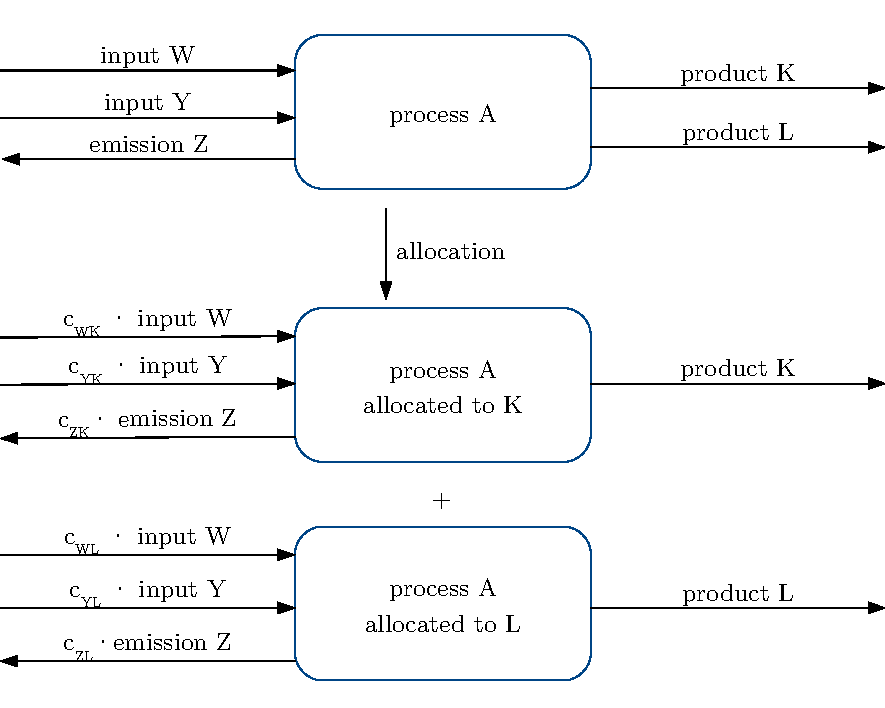
\includegraphics[]{images/allocation.pdf}
    \caption[Allocation]{Allocation is one attempt to solve the multi-output problem in LCA. In this example, process A has two product outputs: K and L. To assign the input flows W, Y and the emission Z to the product flows, the input flows and emissions are partitioned with allocation factors $c_{WK}$, $c_{YK}, c_{ZK}, c_{WL}, c_{YL}$ and $c_{ZL}$. Allocation factors are based on mass, energy or economic price of the output products \cite{InternationalOrganizationforStandardization.2006}. For chemical processes, inputs can be educts, heat or electricity.}
    \label{fig:allocation}
\end{figure}

Conducting a LCA brings some challenges. Chapter \ref{multi-output} presents typical issues and common practices to solve the challenges. Furthermore, to understand LCA database results, this chapter analyses how methodological choices influence the LCA database results. In this thesis, LCA database results are defined as a database of life cycle inventories or impacts of products. This thesis focuses on the methodological choices allocation and cut-off.


\paragraph{Multi-output problem} In general, industrial processes produce numerous products. Inevitably, to run the process, numerous input flows are necessary. Also, a variety of emissions and wastes are produced. Hence, an inventory for the process would have several products. However, LCA practitioners are interested in the inventory per functional unit, which often is related to the product instead of the process. In this case, the practitioner needs to assign the inventory to the products \cite{InternationalOrganizationforStandardization.2006}. The subsequent paragraphs present two approaches to handle the multi-output problem.

\paragraph{System expansion}In order to solve the multi-output problem, ISO 14040 \cite{InternationalOrganizationforStandardization.2006} recommends to expand the product system and to include all product outputs of the process into the functional unit. However, in some cases, this may not align with the goal of the LCA study.

\paragraph{Allocation}
Figure \ref{fig:allocation} illustrates the procedure of allocation. In the allocation approach, the process inputs, emissions and waste flows are mathematically partitioned between all product outputs of the process. Partitioning the flows can be based on the relation of mass, energy or economic prices of the products  \cite{InternationalOrganizationforStandardization.2006}.



\paragraph{Implications of Allocation} With the tools of natural science, it is only possible to quantify inventories of a multi-output process. However, allocating the result to a product requires to partition the inventory. Because the inventory is only defined for the process, there is no objective right way to allocate. Furthermore, partitioning always is a value choice how to choose the allocation factor. When doing allocation based on mass, energy or price, in general the inventories differ. Thus, the allocation factor influences the LCA database results.

Chlorine production is an example for how implementing allocation introduces challenges into the LCA. Chlorine is produced in the chlor-alkali process, a decomposition of sodium chloride solution into chlorine, sodium hydroxide solution and hydrogen  \cite{Du.2018}. Thus, to build an inventory of chlorine, allocation to the three products is performed. First energy allocation based on the enthalpy of formation is considered: elements have a standard enthalpy of formation of zero. In the chlorine example, the allocation factor of chlorine and hydrogen is zero, because they are elements. Thus, all inventories and impacts of the process and its supply are allocated to sodium hydroxide. Considering energy allocation based on the heating value instead for allocation is suitable for hydrogen. However, chlorine and sodium hydroxide are typically not burned for energy production. Thus, this attempt is not applicable here.

In a second attempt, allocation based on mass is chosen. In the process, hydrogen, sodium hydroxide and chlorine are formed in the mass ratios 1.3 \%, 52 \% and 46 \% \cite{Hischier.}. Thus, in this example, allocation based on mass results in a complete different result compared to allocation based on energy.

As mentioned in the introduction (Chapter 1), there are methods to calculate the life cycle inventory of chemical processes. In general, these methods are afflicted with errors. In particular, the amounts of output products a process are erroneous. When allocating the flows to the products based on mass, the error of the output masses propagates to all other flows in the inventory.

\paragraph{Cut-off}
LCA practitioners face the problem of a vast amount of inventory data to collect. Therefore, cut-off is implemented to reduce data requirement. Inventory flows, which have a minor contribution to the LCA result are excluded from the inventory. To distinguish which flowss are relevant in practice, a threshold can be defined. The threshold can be a share of mass or energy of the inventory. Then, all the largest flows, which contribute together as much as the threshold of the inventory,  are considered in the inventory. The smaller flows are cut-off. Also, a cut-off criterion based on environmental significance can be defined. In any case, the cut-off criterion has to be documented in the scope definition of the LCA \cite{InternationalOrganizationforStandardization.2006b}.
 
\paragraph{Implications of cut-off}  When the LCA excludes mass flows, the inventory gets smaller. Thus, the LCIA result is rather underestimated; in any case, never overestimated. When the cut-off is done properly, the implications are minor. To do the cut-off properly, there are critical flows to consider. Even small amounts of critical flows can contribute significantly to the LCIA result. Possibly, the mass flow is below the cut-off limit, but has a relevant impact nevertheless. To prevent an underestimation of LCIA results because of cut-off of critical flows, special care has to be taken.
%Additionally, it has to be considered that cut-off changes the system boundary \cite{InternationalOrganizationforStandardization.2006b}.

\section{\acl{LCA} Database Structures}

\begin{figure}[h!]
    \centering
    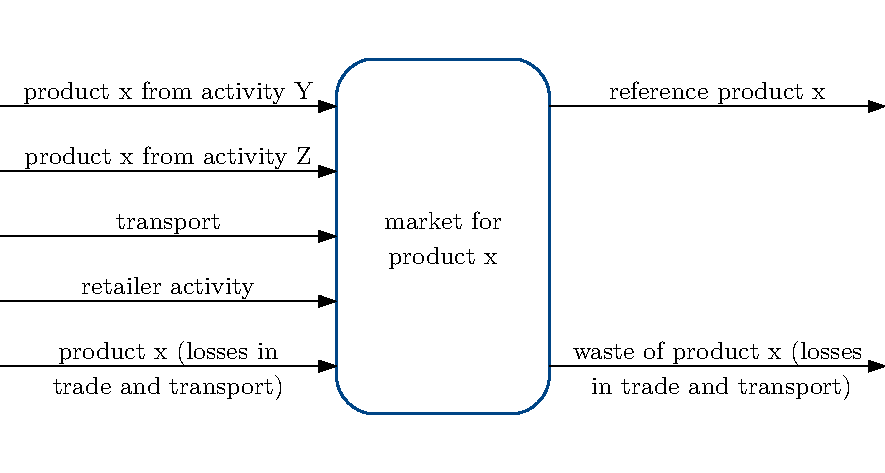
\includegraphics[]{images/market-dataset.pdf}
    \caption[Market dataset in Ecoinvent]{Market dataset in Ecoinvent version 3, which is defined by its name and its inputs and outputs. Adapted from \url{https://www.ecoinvent.org/files/faq_-_market_activity_ecoinvent_3.png}, accessed on March 14, 2020.}
    \label{fig:market}
\end{figure}
\ac{LCA} databases help LCA practitioners to find life cycle inventories or impacts. Thus, databases play an important role in LCA \cite{Wernet.2016}. To understand how  LCA databases are affected by using \aclp{spdm}, this chapter analyses LCA database structure and  generation as well as how LCA database results are affected by the database structure. The LCA database structures are explained on the example of Ecoinvent \cite{Ecoinvent.2020}, a commercial LCA database.

In this thesis, the entries of inventories or impacts for a multitude of chemicals, which are organized in a database, are described by ``LCA database results''. The model of the production network that is used to generate the LCA database results, is described by ``production network model''. LCA database results and the production network model together are described by LCA database. 

The structure of the Ecoinvent database reflects this distinction. Ecoinvent consists of several database layers. In the consumer interface layer, the database customer can access life cycle inventories or impacts results of products. In a second layer, the database calculation layer, life cycle inventories are calculated  \cite{Frischknecht.2007}.

\begin{figure}
    \centering
    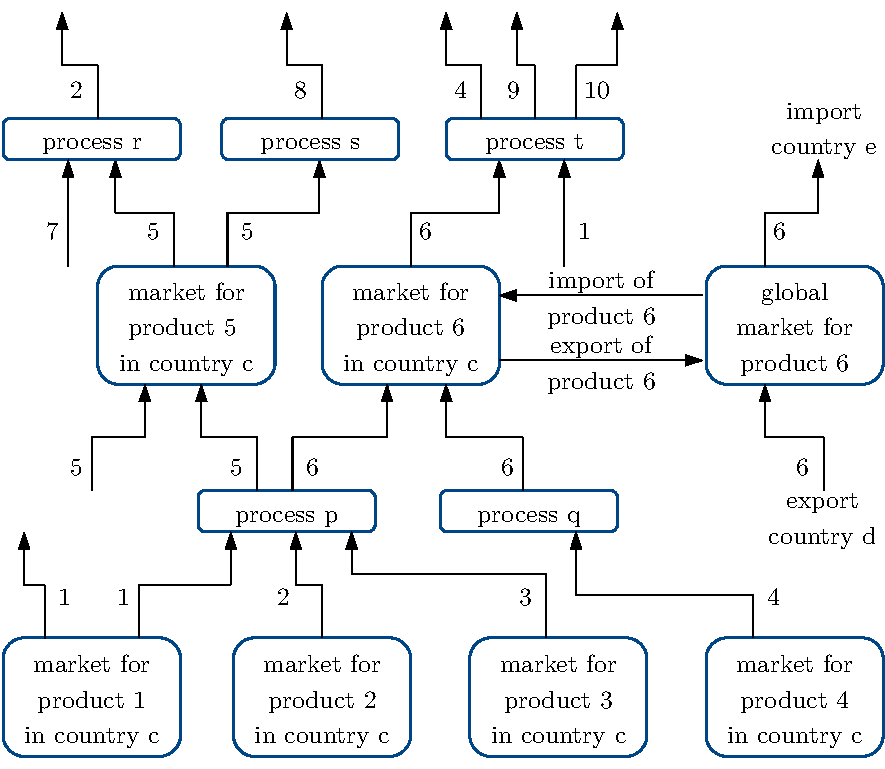
\includegraphics{images/LCA-database.pdf}
    \caption[Production network model]{The production network consists of interconnected production and trade activities that form a global network. This schematic illustration only accounts for the part of the network that is located in country c. The processes p...t each transform  educts into products, wastes and emissions. To keep overview, waste and emission are not depicted. Also, only one global market is depicted, even though all products are traded globally.}
    \label{fig:production-network}
\end{figure}

\paragraph{Production network model}LCA databases model the production network.  This network consists of production activities that are interconnected with each other via intermediates. Each production  activity produces intermediates that are educts for different consecutive production activities. Furthermore, production activities happen in different countries that trade products and intermediates, expanding the network to global size. The sum of all production and trade activities together form a dense network of activities. After several steps, the output of the production network are the final products.

\paragraph{Production activities}All activities in Ecoinvent are represented by datasets with input, output and the name of the activity \cite{Wernet.2016}. Examples for activities are production, transport or market. Production activities are represented by production datasets. Characteristically, chemical production datasets have different inputs and outputs, because a reaction takes place that transforms educts into products.

\paragraph{Market activities}
When modeling a production network, it is important to consider the contribution of a specific production activity to the supply chain. This is necessary in two cases: first, if a product is produced by several production technologies, and second, if the production happens in more than one region. In Ecoinvent, market activities implement both considerations. Figure \ref{fig:market} illustrates the structure of a market dataset in Ecoinvent. Market dataset consists of several inputs and outputs: inputs are flows of the product x from the activity W, Y, Z as well as for compensation of losses in transport;  additional inputs are activities of the retailer. The reference product x and losses from trade and transport are listed as outputs of the market datasets in Ecoinvent. Examples for losses during transport and trade are electrical losses in electricity wires or leakages in chemical pipelines  \cite{Wernet.2016}.  The share of production activities W, Y, Z is named production mix.

The production network is modeled based on consumption mixes. Each educt necessary for a production activity is a mixture of equal educt substances, which are of regional and imported origin.  The consumption mix is calculated by adding the production and import, followed by subtracting the export \cite{Wernet.2016}. The consumption has to be calculated separately for every geographic region that is included. This calculation is based on the assumption that the amount of stored products in the geographic area is stationary in time. In this thesis, consumption mixes are also called market mixes.

\paragraph{Implications of production mixes and consumption mixes for generating LCA databases}

Implications for inventories or impacts occur from the quality of production mix and market mix data: if a product is produced by several technologies with highly different impacts, the accuracy of production mix and market mix data strongly influences the  LCIA result. For example,  the life cycle impact of electricity differs depending on the geographic region. Thus, the impact of the same technology may significantly differ from one region with a large share of renewable energy to a region with a large share of fossil generated electricity. For production technologies with similar impacts, uncertainties in production mix and market mix data have smaller influences.

\paragraph{Regional coverage}
Reasons to implement regional geographical coverage in datasets are: regional geographic coverage takes into account that impacts are counted in the region where they occur. Besides that,  production technology differs in regions of the world. These differences in technology change the inventory -- and thus also the LCIA result. Hence, these differences in the LCI and LCIA results are covered in regionalized datasets \cite{Wernet.2016}. Ecoinvent generates geographic datasets in the following manner:  usually, Ecoinvent offers one global dataset, derived from global production information. In case of regional datasets additionally being available, a ``rest of the world'' dataset is generated. The rest of the world dataset is calculated from the difference between the global dataset and the sum of all regional datasets.

\paragraph{Multi-output problem in Ecoinvent}The multi-output problem (see Chapter \ref{multi-output}) also occurs in the Ecoinvent database. In the undefined system model, Ecoinvent models activities instead of products. Ecoinvent offers three system models to handle the multi-output problem. The first system model applies allocation, the second one system expansion and the third one a combination of both  \cite{Wernet.2016}. See illustration of allocation in Figure \ref{fig:allocation}.

\paragraph{Supply processes} When building new LCA databases, it is possible to model the complete production network from raw materials to final products. However, the complete scope requires more modeling efford than focusing on relevant parts of the production network. For example, it might be sufficient to exclude the electricity production from the production network model for a chemical LCA database. 

Nevertheless, the downsized production network model needs inputs of materials and energy that are produced outside of the production network model. To supply the production network model with input materials or energy, inventory or impact datasets from other databases can be integrated. The datasets are ``aggregated datasets'' as they aggregate several unit processes into one dataset. In this thesis, aggregated datasets that are used to supply the production network model with products, which are outside of the scope of the production network, are called supply processes. 

Ecoinvent also lists aggregated datasets. One example is the  Ecoinvent LCIA dataset ``market for electricity, high voltage, DE'' \cite{TreyerK..}. This dataset lists the impacts that arise from the production and delivery of 1 kWh of electricity in Germany. The LCIA data customer does not need to have knowledge about the unit processes of electricity production and the electricity market in Germany.

\paragraph{Implications of supply processes for generating LCA databases}
Implications of supply processes on LCA database results depend on the available data. The supply processes should cover technology shares in the concerned region adequately. In chemical production networks, important flows that have to be supplied are electricity, heat and the educts that enter the production network. As Chapter \ref{spdm} describes, \aclp{spdm} only calculate the heat demand but not the ratio of fuels and other heat sources. Due to a lower carbon content, heating with natural gas has a lower global warming impact than coal for instance. Thus, the choice of heat supply mixes influences the LCIA result of the chemicals produced in the production network. 



\chapter{Simplified Process Design Methods}
\label{spdm}
The term ``simplified process design methods'' is used here to describe inventory generation methods from literature (\cite{Parvatker.2019, Hischier.2005, Perry.1999, Smith.2017, JimenezGonzalez.2000}), that are based on chemical process engineering, but rely on little data input for calculation.

The goal of this chapter is to qualitatively understand the influence of using \acl{spdm}s on inventory components and on selected impact categories. A generic model of chemical processes reveals which inventory components are relevant in context of chemical processes. Later, this thesis introduces and evaluates \acl{spdm}s to calculate inventories for chemical unit processes. The results of the evaluation are summarized in Table \ref{tab:spdm}, at the end of the chapter.

\section{Simplified Model of Chemical Processes}
\label{simplified-model-processes}
To assess which inventory components enter and leave the system of a chemical process, a simplified model of chemical processes is used. %Later, in chapter \ref{analysis-spdm}, the \acl{spdm}s are presented and analysed with regard to generating the inventory components.
Also, the case study in chapter \ref{chap:case study} is calculated on the basis of the simplified model of chemical processes.

%Figure: Flow Sheet
\begin{figure}[htp]
        \centering
        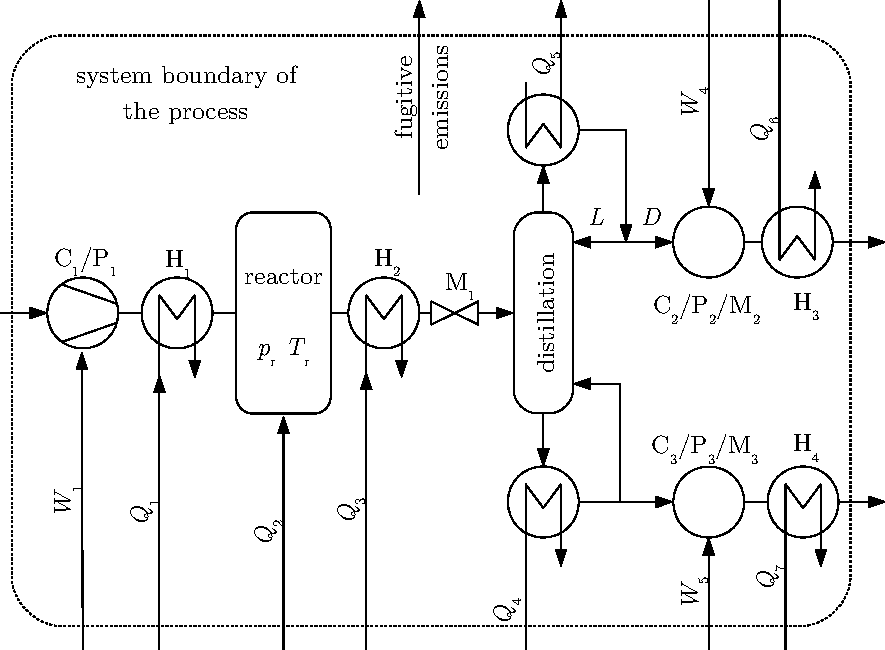
\includegraphics[width=\textwidth]{images/flow_sheet.pdf}
        \caption[Generic flow sheet]{Generic flow sheet: This flow sheet illustrates how chemical processes are simplified in this thesis. $p_r$ and $T_r$ are reaction pressure and temperature, C$_i$ are compressors, P$_i$ pumps and M$_i$ chokes, H$_i$ are heat exchangers, $L$ is the reflux flow, $D$ the distillate flow, $W_i$ are electrical works and $Q_i$ are heat flows.}
        \label{fig:flow sheet}
\end{figure}

\paragraph{Industrial chemical processes}
In general, industrial chemical processes comprise a complex network of chemical engineering operations: a heat exchangers network, several reactors, pumps, compressors, distillation columns, filters, dryers and chokes. 

\paragraph{Flow sheet}To describe the sequence of operations in chemical processes, flow sheets were developed. Flow sheets show all process equipment and how it is interconnected. Designing the flow sheet of industrial chemical processes is the field of process design engineers and requires a large amount of resources, such as time and knowledge. Every chemical process has its own flow sheet  \cite{Douglas.1985}. 

For the generation of inventory data of chemical processes, it is essential to know the sequence of unit processes. Thus, the flow sheet is the basis for later calculation of inventory data.  

\paragraph{Generic flow sheet} Because industrial processes have unique flow sheets and the automated generation of flow sheets is challenging, this thesis uses a simplified generic flow sheet for generating LCA databases. Figure \ref{fig:flow sheet} illustrates this generic flow sheet. The generic flow sheet considers the minimum equipment to perform chemical reactions: heat exchangers, compressor/pumps, one reactor and one distillation column.

On the left side of the flow sheet, educts enter the chemical process. The educts are first compressed to reaction pressure. For gaseous educts, the compression is done by the compressor C$_1$; for liquid educts by the pump P$_1$. Compressor or pump are driven by mechanical work $W_1$, which is ether supplied by a turbine, engine or electric motor. The compressor is followed by the heat exchanger H$_1$ that conditions the educts to reaction temperature. To change the temperature, heat $Q_1$ is introduced. In the next step, the educts pass the reactor and convert partially at reaction condition ($p_r$ and $T_r$). For endothermic reaction, heat $Q_2$ has to be introduced to maintain reaction temperature $(Q_2>0)$, exothermic reactions release heat that has to be dissipated $(Q_2<0)$. According to Douglas \cite{Douglas.1985}, industrial reactors have an educt recycling loop: unreacted educts are separated and feed back into the entrance of the reactor. In this thesis, it is assumed that the industrial reactor, separator of unreacted educts and recycling loop is replaced by the generic reactor. The generic reactor lacks the educt recycling, however considers the effect of the educt recycling by a higher conversion. Nevertheless, the generic reactor outputs unreacted educts and non-products, which are considered as waste. The heat exchanger H$_2$ and the choke M$_1$ follow, which bring the reactor outlet mixture to distillation conditions. The heat exchanger is supplied with heat $Q_3$. The choke is assumed to be adiabatic here. In the distillation column, the product is separated from waste. To perform the distillation, $Q_4$ is introduced at the bottom of the distillation column and $Q_5$ is dissipated at the top. After the distillation column, the choke M$_2$, the compressor C$_2$ or the pump P$_2$ brings the product to atmospheric pressure. A choke is used if distillation pressure is higher than atmospheric pressure, otherwise a compressor or pump is used. To run the compressors or pumps, the work $W_4$ is necessary. Consecutively, the heat exchanger H$_3$ brings the product to standard temperature. The bottom output of the distillation is ether a second product, waste or a mixture, which is separated in a second distillation column. In the case of a product or waste, the compressor C$_3$, the pump P$_3$ or the choke M$_3$ ensure that the flow leaves the system at atmospheric pressure. The heat exchanger H$_4$ brings the flow to standard temperature.  To keep the overview, fugitive emission sources are unlocated in the flow sheet; all equipment with leakages can emit fugitive emissions. 

%\paragraph{Limitations}The simplified model has limitations of products. For instance, the extracrion of salts from water need crystalization. As there is no crystalizer in the generic flowsheet, salt production cannot be modeled. Due to the above simplifications regarding the number of equipment, there are uncertainties of transferring results obtained from the simplified model to industrial processes.

\paragraph{Inventory components}The inventory of the generic chemical process is a list of flows, which cross the system boundary. In the generic flow sheet (Figure \ref{fig:flow sheet}), mass flows of educts, the product, fugitive emissions as well as flows of work $W_i$ and heat $Q_i$ cross the system boundary. In this thesis, four categories of inventory components are introduced: 
\begin{itemize}
    \item Mass flows are the flows of educt, products and waste;
    \item Electricity, as it is assumed that electricity provides work $W_i$;  
    \item Steam, fuel and other sources of heat are aggregated as heat;
    \item Emissions of substances from equipment leakages are summarized as fugitive emissions.
\end{itemize}

\section{Simplified Life Cycle Impact Assessment Methodology}
\label{chap:lcia-meth}
Chapter \ref{analysis-spdm} evaluates qualitatively how \aclp{spdm} influence the life cycle impact of chemicals. Initially, \aclp{spdm} calculate the inventory. To generate qualitative life cycle impacts from the inventory a simplified LCIA methodology is introduced. Two impact categories are chosen: global warming impact and toxicity. %Yet, Calvo-Serrano et al. found that the impact category ``cumulative energy demand'' is correlated with global warming impact \cite{CalvoSerrano.2018}. Thus, in the following considerations, global warming impact also represents the cumulative energy demand.
The assignment from inventory components to life cycle impacts is:
\begin{itemize}
    \item Electricity and heat: according to the US Energy Information Agency \cite{U.S.EnergyInformationAdministration.202003}, in 2019,  63\% of the energy consumed by the industrial sector in the US was generated by fossil fuels. Due to the fact that the production of heat and electricity from fossil fuels emits CO$_2$, electricity and steam contribute to the global warming impact in this LCIA methodology.
    
    Similarly, the burning of  fossil fuels emits toxic substances \cite{FitzGerald.}. Thus, energy production contributes to the toxicity impact in this simplified LCIA method.
    \item Fugitive emissions: it is assumed that the mass flows within a process are toxic. Therefore, leakages emit traces of toxic substances into the environment. Thus, mass flows contribute to toxicity impacts.
    \item Mass flows: input materials for chemical processes are products of previous chemical processes. The previous processes are burdened with global warming and toxicity impacts. %Also waste that is formed in a chemical process is treated, which requires energy and releases emissions. The impacts of the waste treatment are assigned to the chemical process, as waste treatment is a mandatory part of the life cycle.
    Thus, educt mass flows contribute to global warming and toxicity impacts of the process.
\end{itemize}

\section{Analysis of Simplified Process Design Methods}
\label{analysis-spdm}

The goal of this chapter is to introduce \acl{spdm}s from literature and to qualitatively understand the effect of using \aclp{spdm} on inventory components (Chapter \ref{simplified-model-processes}) and on impacts, using the simplified LCIA methodology (Chapter \ref{chap:lcia-meth}). This thesis focuses on the impact categories ``global warming impact'' and ``toxicity''. 


\subsection{Mass Flows based on the Stoichiometric Equation}
\label{stoichiometry}
The stoichiometric method is a widely used \acl{spdm} in the LCA database Ecoinvent: In version 2.0 of the database, more than half of the inventories of chemicals were generated by the stoichiometric method \cite{Althaus.2007}.

Stoichiometry is used to calculate the input and output mass flows of a chemical reactor \cite{Parvatker.2019} (see reactor in flow sheet Figure \ref{fig:flow sheet}). The basis of the calculation is the balanced stoichiometric equation \[ \sum{\nu_i E_i} \rightleftharpoons \sum{\nu_j P_j},\] with educts $E_i$ and products $P_i$ and  the stoichiometric coefficients $\nu_i$. For using this method, besides the stoichiometric equation, the molar masses of all substances of the reaction have to be known. Then, applying a stationary mass balance around the reactor, the masses of educts, products and waste can be calculated. This serves as inventory for the LCA.\\

%The input to the reactor is \[\nu_i mol\] of every educt, the output is \[\nu_j mol\] of every output of process. molar inventory per desired product: inputs:\[\frac{\nu_i{ mol}}{\nu_P{}mol}\] and outputs \[\frac{\nu_j mol}{\nu_P mol}\]ratios reactants, target chemicals, products \cite{pavatker.2019}: combined with molar weight : respective mass flows, 

%The assumption that a chemical reaction that follows the stoichiometric equation is a good assumption, as long a the stoichiometric equation accounts for all possible side reactions at reaction conditions. However, equilibrium reactions do not convert completely. Thus besides the products there are still significant amounts of educt in the reactor output. To obtain more realistic results, it is possible to  
To evaluate the stoichiometric method, a realistic reactor in industry is compared to a stoichiometric reactor. Industrial reactors often do not use educts in the stoichiometric relation. Instead, one educt is used in excess \cite{Piccinno.2016}. Reasons for excess use are less formation of unwanted side products and a faster conversion \cite{Luyben.2000}. Inevitably, the reactor output still contains much of the excess educt and possibly other unreacted educts in case of equilibrium reactions. Thus, the inventory of an  industrial reactor has more educt input and output than the stoichiometric equation suggests. However, chemical plant operators do not waste the unreacted educts. As explained in Chapter \ref{simplified-model-processes}, industrial reactors are followed by an educt recycling. Because of the circulation of unreacted educts in the recycling loop, the unreacted educts are fed back to the reactor. Assuming a perfect educt recycling without waste, all the outputs of the generic reactor are present exactly in the stoichiometric relation. This can also be seen by performing a mass balance around the reactor with educt recycling. 

Because of the complex calculation of the output composition of a realistic reactor with educt recycling, the educt recycling is not illustrated in the flow sheet (Figure \ref{fig:flow sheet}). The effect of educt recycling is modeled through the ideal, generic reactor. The ideal generic reactor in the flow sheet \ref{fig:flow sheet} replaces a realistic reactor plus educt recycling. For the generic reactor, the educt recycling is replaced by the assumption of stoichiometric input and output flows. On the one hand, this consideration justifies the use of the stoichiometric method.\\%  Thus, assuming a high yield for the generic reactor in this thesis is justified. The results of the mass flow a inventory thus should come close to industrial inventories.\\

On the other hand, it is difficult or economically unfeasible  \cite{Douglas.1985} to separate all the unreacted educts. Thus, the educt recycling is incomplete; a part of educts becomes waste. The more educts are wasted, the more the stoichiometric equation underestimates the inventory. This consideration limits the use of the stoichiometric method.

Incorporating a yield  \cite{Parvatker.2019} to the stoichiometric method aims to offset the influence of waste formation in the process. Yield is defined as the ratio of the obtained amount of product and the theoretical, maximal possible amount of product  \cite{Christen.2010}. The implication of using the stoichiometric method with yield highly depends on the certainty of the yield. If the assumed yield is higher than the real yield, an underestimation of material inventory occurs and vice versa. Hischier et al.  \cite{Hischier.2005} suggests to use a yield of 0.95\footnote{In the source \cite{Hischier.2005}, an efficiency of 0.95 is suggested. It is assumed here that efficiency equals yield.}.

In real chemical reactions, additional ancillary materials are present. Examples of ancillary materials are catalysts and solvents. Depending on the process, solvents and catalysts may be recycled, otherwise wasted after use  \cite{Piccinno.2016}. Thus, a contribution for solvent and catalyst supply and waste treatment to the inventory is assumed. However, ancillary materials are omitted in the stoichiometric method, thus the inventory is underestimated. Evaluating the consequences of the underestimation is difficult, because the amount of solvents and catalysts in relation to the product differ with the specific reaction. In addition, the ecological significance of ancillary materials differ. If ancillary materials have an environmental significance, the impact is underestimated. 

As the stoichiometric method does not calculate energy requirements of the reaction, the energy requirement for operating the educt recycling is not considered in the inventory. Thus, the use of the stoichiometric method contributes to an underestimation of the energy demand of the reaction, if the educt recycling is not modeled with another method. 

To summarize the implications of using the stoichiometric method for the generation of material inventories, an underestimation due to the exclusion of waste is expected. Thus, with the simplified LCIA methodology, an underestimation of global warming impact and toxicity is expected. The exclusion of the energy requirement for educt recycling in the stoichiometric method contributes to an underestimated energy requirement of the product. Incorporating a yield $<1$ into the method may correct the underestimation; or may even change the underestimation to an overestimation.

\subsection{Energy Values of the Ecoinvent Approach}
\label{gendorf}
Ecoinvent has established a method for generating the energy inventories and emissions of chemical processes. According to Hischier et al. \cite{Hischier.2005}, the full method also consists of the stoichiometric method. As stoichiometry is subject of chapter \ref{stoichiometry}, this Chapter focuses on the generation of energy inventories and Chapter \ref{gendorf-emission} on emission inventories.

%Applied to the generic flow sheet (Figure \ref{fig:flow sheet}), the energy inventory part of the ``Ecoinvent-method'' estimates the sum of all heat flows $Q_i$ and the sum of all electricity demands $W_i$. Thereby, t
The Ecoinvent-method takes the average electricity and fuel consumption -- used for the production of chemicals -- as default values for the energy inventory.  The average is calculated from the environmental report of the chemical plant in Gendorf, Germany \cite{GendorfChemiepark.2000}. The Gendorf plant produces approximately 1500 chemical products  \cite{Hischier.2005}.

The calculated average values for energy and fuel consumption are used as default values in the inventory of chemicals. It is assumed that the electricity is used to run process auxiliaries and waste water treatment. Thus, the Ecoinvent-method estimates the energy consumption $\sum W_i$ of the pumps or compressors in the generic flow sheet \ref{fig:flow sheet}. Fuels are assumed to deliver heat for preheating of chemicals and for distillation  \cite{Hischier.2005}. Therefore, the Ecoinvent-method approximates the sum of all heat flows $\sum Q_i$.

Approximating the energy demand with default values is a simplification. Therefore, process specific properties are excluded from consideration. Examples for process specific properties that affect the electricity demand are the process pressures.  The fuel consumption, for instance, is influenced by the process specific property, if the reaction is endothermic or exothermic.

To sum up, the default values are an estimation of the energy demand. It is unpredictable whether the default values approximate the real energy consumption properly or  under- or overestimate it. According to the simplified LCIA methodology (Chapter \ref{chap:lcia-meth}), an under- or overestimation of the global warming impact and toxicity is possible.

%between cradle to gate and gate to gate
%Doppelgendorf (Nachschauen in gendorf umwelterklärung energiebedarf und dann mit Ecoinvent paper vergleichen)




\subsection{Heat Requirement of Reaction, based on Reaction Enthalpy}
\label{enthalpy}
The reaction-enthalpy-method is a basic model for the energy requirement of a reactor. In the flow sheet (Figure \ref{fig:flow sheet}), the method calculates the heat $Q_2$. Within the reaction-enthalpy-method, the heat of reaction is taken as an approximation for the heat requirement of the reactor. The heat of reaction can, for instance, be calculated from the heat of formation  \cite{Parvatker.2019}. The heat of formation is material-specific and can be accessed in chemical property tables.

The scope of the reaction-enthalpy-method simplifies the energy requirement or a reactor: reasons for energy consumption are only partly covered. For instance, heat losses and energy for stirring are excluded in the calculation. According to the reaction-enthalpy-method, endothermic reactions result in heat output. The heat is collected with heat recovery, which has a limited efficiency. Percentages of possible heat recovery depend on the temperature of the reactor  \cite{JimenezGonzalez.2000,Branan.2002}. The higher the temperature, the more heat can be recovered.%At low temperatures, usually the energy from the endothermic reaction is dissipated with cooling water.\\

An advantage of the reaction-enthalpy-method is the little data input that is necessary for the calculation. The reaction-enthalpy-method alone underestimates the energy requirement of a reactor, as it excludes reasons for energy requirement. Thus, global warming impact and toxicity are also underestimated.

\subsection{Heat Required for Temperature Change}
\label{heatup}
The  temperature-change method calculates the energy inventory to heat substances from one temperature level to another.  Applied to the generic flow sheet, the temperature-change method calculates energy demand of the heat exchangers H$_i$ in the generic flow sheet (Figure \ref{fig:flow sheet}). To calculate the energy demand, the temperature difference is needed. Also, information about the heat capacity is necessary. According to Piccinno et al. \cite{Piccinno.2016}, the heat demand $Q_i$ is 
\begin{equation}
\label{equ:temper}
    Q_i=mc_p\Delta T,
\end{equation}
with the heated mass $m$, the isobaric heat capacity $c_p$ and the temperature difference $\Delta T$.

According to Baehr et al. \cite{Baehr.2016}, Equation \ref{equ:temper} incorporates the assumption of an ideal fluid with constant heat capacity; additionally, for the case of a liquid, an isobaric heat exchanger. Also, heat losses are excluded of the analysis, but occur in real heat exchangers. These assumptions have to be justified for the application.

If the temperature is decreased in the heat exchanger, it has to be considered that only a fraction of the heat can be recovered for reuse. This especially applies for low temperature  \cite{JimenezGonzalez.2000,Branan.2002}.

Calculating the energy demand of heating is a standard process design task. Thus, this method is supposed to deliver reliable results for energy inventories and its connected impact category global warming impact and toxicity.

When the temperature-change method is applied to the heat exchanger supplied by $Q_1$, it calculates the energy demand to condition the educts from ambient to reaction temperature. Together with the reaction-enthalpy-method (Chapter \ref{enthalpy}), two causes of the energy demand of reactors (reaction enthalpy and condition) are considered. This serves as a basis for energy inventory calculation of reactions in literature \cite{Parvatker.2019}.





\subsection{Heat Requirement of Distillation by Piccinno et al.}
The distillation method by Piccinno et al. calculates the energy requirement to separate one product.  In the generic flow sheet (Figure \ref{fig:flow sheet}), the energy inventory for distillation is represented by the %heat $Q_3=Q_{heat}$ for heat up to distillation temperature and 
heat $Q_4$ at the bottom of the distillation column to vaporize the liquids.  Heat $Q_5$ is dissipated at the top to condense the product and is assumed to be wasted. Piccino et al. \cite{Piccinno.2016} suggest equation \ref{equa:distil} based on the heat of vaporization:

\begin{equation}
\label{equa:distil}
    Q_4=Q_{dist}=\frac{\Delta h_{vap}m_{dist}\cdot(R+1)}{\eta_{heat}-0.1}. %only R
    %Q_{dist}=\frac{Q_{heat}+Q_{vap}\cdot(R+1)}{\eta_{heat}-1}=\frac{c_pm_{mix}(T_{boil}-T_0)+\Delta h_{vap}m_{mix}\cdot(R+1)}{\eta_{heat}-0.1}. %only R
\end{equation}

In Equation \ref{equa:distil}, $Q_{dist}$ is the heat demand of the distillation,  %$c_p$ is the isobaric heat capacity,
$m_{dist}$ is the mass of the distillate, the head product of the distillation, %$T_{boil}-T_0)$ the temperature difference between distillation inlet and reactor outlet, 
and $\Delta h_{vap}$ is the enthalpy of vaporization. %Calculation of the heat demand to reach the boiling point of the mixture follows the method in chapter \ref{heatup} and delivers \(Q_3=Q_{heat}=c_pm_{mix}(T_{boil}-T_0)\). 
Because of the reflux, a part of the head product is condensed and fed back to the distillation column to be reboiled. The amount of fed back product is described by the reflux ratio $R$, which is reflux flow $L$ divided by the distillate flow $D$. To approximate heat losses, the heating efficiency $\eta_{heat}$ is reduced by 10\% in the formula \cite{Piccinno.2016}.%Distillation does only work, if reflux ratio exceeds the minimum reflux ratio ($R\geq R_{min}$). $R_{min}$ is calculated by the Underwood equation \cite{Piccinno.2016} \[R_{min}=\frac{1}{1-\alpha}\left(\frac{x_{LD}}{x_{LF}}-\frac{\alpha (1-X_{LD})}{1-X_{LF}}\right), \]in which $\alpha$ is the relative volatility, and $x_{LD}$ the traget purity of the distillate and $x_{LF}$ the traget  To ensure, that $R>R_{min}$, the factor 1.2 was introduced in formula \ref{equa:distil}.
 
The energy demand to reach a certain distillation pressure is ignored here, as industrial distillation happens usually under ambient pressure. Exceptions are cases with substances with high boiling points (approximately >200\degree C) or very similar boiling points in the reactor outcome. Anyways, the method is initially developed for batch processes  \cite{Piccinno.2016}, which may limit the accuracy for stationary processes.

The method introduced accounts for all important energy demand in distillation: heat of vaporization and heat losses. The method has a low data requirement: the distillation temperature and additional assumptions for the reflux ratio $R$ and the heat efficiency $\eta_{heat}$. The quality of the energy inventory result depends on choices of the last two parameters. For proper parameters, the distillation method by Piccinno et al. is supposed to generate realistic inventories. Inappropriate parameters may result in an over- or underestimation of the energy requirement and consequentially of the global warming impact and toxicity impact.

\subsection{Energy Requirement of Pumps based on Piccinno et al.}
For liquid reaction processes, this method can be applied to approximate the energy requirement of pumps (see pumps P$_i$, flow sheet Figure \ref{fig:flow sheet}). The energy demand of a pump depends on a variety of physical influences: the height difference, the speed difference of the liquid between pump inlet and outlet, the friction in the pipe to the next equipment and the static pressure drop in the equipment after the pump. Piccinno et al. \cite{Piccinno.2016} quantify the energy demand by
\begin{equation}
\label{equ:pump}
    E_{pump}=\frac{m}{\eta_{pump}}\cdot \left( \Delta h_{equip} \ g+\frac{\Delta v^2}{2}+\frac{\Delta p}{\rho}+\frac{\lambda lv^2}{2d}\right).
\end{equation}


The parameters are mass $m$, efficiency of the pump \(\eta_{pump}\), height difference between pump and equipment inlet $\Delta h$,  gravitational constant $g$, difference in speed between pump inlet and outlet $\Delta v$, static pressure drop in the equipment after the pump $\Delta p_{equip}$,  density of the liquid $\rho$, friction factor $\lambda$, length $l$, diameter $d$ of the pipe and speed of the liquid in the pipe $v$.

Unfortunately, many of those parameters are equipment-size-specific and thus difficult to collect in the scope of fast and automated LCA database generation. Also, friction in pipes is not considered in this thesis. Therefore, Equation \ref{equ:pump} can be simplified by assuming friction free flow, no speed difference between inlet and outlet of the pump and no height difference of equipment:

\begin{equation}
\label{equ:pumpsimple}
    E_{pump}=\frac{m}{\eta_{pump}}\cdot\frac{\Delta p}{\rho},
\end{equation}


%On the one hand, the parameters enable a process specific energy inventory of a pump. On the other side, collecting all parameters can be challenging for a LCA database with a vast amount of chemicals.  If parameter data is not available,  \cite{Piccinno.2016} lists default values for a generic process for parameters in the formula which result in an energy demand per transfered mass of\(55 \frac{J}{kg}\) for every pump, finally. This simplification reduces the data intensity. However, with this simplification the energy inventory only accounts for the number of pumps in the process, but not to the pressure drop and the pump efficiency anymore. Thus, the simplification is only partly process specific and thus assumed to be inaccurate.

where $\Delta p_{pump}$ is now the static pressure difference between pump outlet and inlet. Now, all parameters in equation \ref{equ:pumpsimple} can be derived from the generic flow sheet: with a realistic pump efficiency, the energy inventory is expected to be accurate. Thus, the global warming impact and the toxicity are properly approximated.

\subsection{Energy Requirement of Compressors based on Thermodynamic Considerations}
%Perrys Handbook 1999, page 372 / 2471 or 4-36 thermodynamics  \cite{PerryRobertH..1999}
In gas reaction processes, a compressor is used to increase the pressure instead  of a pump  (compressors C$_i$ in the  generic flow sheet Figure \ref{fig:flow sheet}). This method builds on thermodynamic consideration from Perry's Chemical Engineers' Handbook \cite{Perry.1999}: the fluid is assumed to be ideal and the compression is assumed to be isentropic and completely intercooled after each compressor stage. To include dissipation, a compressor efficiency $\eta$ is introduced. Finally, this yields the equation \[P=\frac{n\gamma RT}{\eta\cdot (\gamma -1)}  \left[ \left(\frac{p_2}{p_1}\right)^\frac{\gamma -1}{n\gamma}-1 \right] \cite{Perry.1999}. \]
Values in the formula are: number of compressor stages $n$, heat capacities $\gamma$ (1.4 for air as ideal gas), temperature $T$, pressure $p$, universal gas constant $R=8.314 \frac{J}{mol K}$, index $1$ before the compressor and index $2$ after the last compressor stage.

This method is easily integrated into LCA databases as it only requires few data. The reliability of the result depends on a realistic value for the efficiency of the compressor. Assuming to know an appropriate efficiency value, this formula is an accurate approximation of the energy requirement of a compressor in a chemical process. Thus, the derived impacts ``global warming impact'' and ``toxicity''  are supposed to be accurate.

\subsection{Fugitive Emissions, based on Empirical Findings by Smith et al. \cite{Smith.2017}}
\label{chap:Smith}
Fugitive emissions occur because of leakages in chemical processes. Smith et al. \cite{Smith.2017} have applied findings about equipment leakages from the United States Environmental Protection Agency  \cite{U.S.EnvironmentalProtectionAgency.1995} to generate life cycle inventory data: 
\[E_T= \sum_{i}n_i \cdot f_i \cdot t\] describes the annual fugitive emission. This equation has to be applied on every single chemical in a process. Within the formula, $i$ is the type of fugitive source (equipment), $n_i$ is the quantity of equipment $i$ in the flow sheet, $f_i$ is the emission factor of equipment $i$ in $\frac{kg}{h\cdot source}$ and $t$ is the operation time in hours per year.

Emissions occur in pumps, compressors, valves, connectors, open-end lines, sampling connection and relief valves \cite{Smith.2017}. Pumps and compressors are the only equipment that is present in the flow sheet Figure \ref{fig:flow sheet}. Therefore, applied to the equipment in the generic flow sheet, the Smith-emission-method only calculates emission inventories for pumps and compressors. The emission factors $f_i$ are introduced in Table \ref{tab:emissionSmith}. Emission factors for equipment that is not existent in the flow sheet, can be obtained from Smith et al, 2017 \cite{Smith.2017}.

\begin{table}[h]
\caption[Average emission factors for equipment in the generic flow sheet by Smith et al.]{Average emission factors for equipment in the generic flow sheet by Smith et al. Light liquids have a vapor pressure higher than 0.3 kPa at 20 °C. Heavy liquids have a vapor pressure below 0.3 kPa at 20 °C (adapted from  \cite{U.S.EnvironmentalProtectionAgency.1995,Smith.2017}).}
\label{tab:emissionSmith}
\centering
\begin{tabular}{ccc}
\toprule
\textbf{equipment type} & \textbf{fluid} & \textbf{emission factor $f_i$ in $\frac{\mathrm{kg}}{\mathrm{h}\cdot \mathrm{source}}$} \\ \midrule
pumps & light liquid & 0.0199\\\
{}& heavy liquid & 0.00862\\
compressors & gas & 0.228\\\bottomrule
\end{tabular}
    
\end{table}

The Smith-emission-method only needs basic data: the quantity of compressors or pumps, the categorization of the vapor pressure in high and low and the material inventory to derive the emissions. The low data requirement makes the method suitable for the fast and automated inventory generation for LCA databases. As the method is based on the environmental report of the Environmental Protection Agency, the factors are supposed to be reliable. 

However, the adaptations of the method in this thesis have excluded emissions from valves, connectors, open-end lines, sampling connection and relief valves. %Thus, this method as it is adapted here, only includes compressor and pumps. 
Because of this limited scope, the method is supposed to slightly underestimate the emission inventory. Therefore, generating LCA datasets with this method will result in a slight underestimation of the derived toxicity impact.

\subsection{Fugitive Emissions Factors of the Ecoinvent Method}
\label{gendorf-emission}
The Ecoinvent-method also estimates fugitive emissions, which are depicted at the top of Figure \ref{fig:flow sheet}. Emissions into the air are assumed to be 0.2 \% of the input materials % Emission to water are assumed to be the difference of unreacted educts and air emission, resulting in 4.8\% of input material
 \cite{Hischier.2005, Althaus.2007}.%Although not mentioned in the Ecoinvent report \cite{Hischier.2005}, some of Ecoinvent datasets use an internal waste water treatment that removes 90\% of the emission from the water \cite{Althaus.2007}. Thus, the emissions to water are reduced to  0.02\%. Solid waste formation is assumed insignificant in liquid or gaseous reactions. Thus, Solid waste are not considered.
Using default emission factors does not reflect different equipment. Still, it is a process-specific assumption: high input of toxic substances result in high emission of toxic material inventory. Nevertheless, the Ecoinvent emission method excludes intermediates and products that are present in the process from the inventory.

In order to understand the ability of the Ecoinvent-method to calculate fugitive emission inventories,
the value of the air emission factor has to be evaluated. Therefore, the Ecoinvent emission factor is compared to the empirical emission factors by Smith et al. \cite{Smith.2017} (see Chapter \ref{chap:Smith}, comparison see Table \ref{tab:comp-fugi-Eco} in the Appendix). The result shows that the Ecoinvent emission factor is at least one magnitude higher than the emission factor by Smith et al. As explained in Chapter \ref{chap:Smith}, the Smith-method slightly underestimates fugitive emissions, thus the Ecoinvent-method still overestimates them. In conclusion, with the LCIA methodology in Chapter \ref{chap:lcia-meth}, the toxicity impact is overestimated by the air emissions of the Ecoinvent-method.


\subsection{Fugitive Emissions based on Rule of Thumb by Jiménez-González et al. \cite{JimenezGonzalez.2000}}
Similar to the method by Smith et al., the fugitive emission method by Jiménez-González generates fugitive emission inventories that originate from equipment leakages. Jiménez-González et al. \cite{JimenezGonzalez.2000} proposes a rule of thumb based on expert judgment, see Table \ref{tab:Jimenez}.

\begin{table}[]
\caption{Fugitive emission factors for the entire chemical process, based on a rule of thumb by Jiménez-González et al. (adapted from \cite{JimenezGonzalez.2000}) }
\label{tab:Jimenez}
\centering
   \begin{tabular}{ccc}
   \toprule
    \textbf{fluid} & \textbf{boiling point} & \textbf{emission factor} \\
            & \textbf{at 1013 hPa }&   \\\midrule
    liquids &  $20...60$ °C   &   2 \%\\
            &   $60...120$ °C &   1 \%\\\midrule
    gases   &   $<20$ °C      &   0.5 \%\\\bottomrule
    \end{tabular}
\end{table}
In contrast to the method by Smith et al., the emission factors by Jiménez-González et al. apply for the entire production process instead of single unit operations. Thus, the method calculates the summed emissions of all equipment in the flow sheet (Figure \ref{fig:flow sheet}). In contrast to the Ecoinvent emission method, which only considers the process inputs, the method by Jiménez-González et al. compiles emissions for all substances present in the production process.

Advantageously, the rule of thumb hardly needs data: only the mass flow inventory and the characterization of the fluids according to the boiling points are necessary. Evaluating the method is difficult, as it is based on expert judgement. However, a comparison of the emission factors by  Jiménez-González et al. and by Smith et al. is possible. The comparison reveals that the factors by Jiménez-González et al. are at least one magnitude higher (see Table \ref{tab:comp-fugi} in the Appendix). Assuming a slight underestimation of the method by Smith et al., the method by Jiménez-González still overestimates the emission inventory and the derived toxicity impact.



\subsection{Summary and Conclusion}

%overview spdm methods table
\begin{table}
\caption[Summary of qualitative implications for life cycle inventory  and impact results when using \acl{spdm}s.]{Summary of qualitative implications for life cycle inventory  and impact results when using \acl{spdm}s. Vertical: \acl{spdm}s, horizontal: inventory components and impacts. ``+'' marks an overestimation by the \acl{spdm}, while ``$-$'' marks an underestimation. ``1'' symbols a proper approximation, ``$\emptyset$'' represents that the method does not influence the inventory component or impact. Behind the symbols, a short comment explains the reason for the over- or underestimation. $R$ is the distillation reflux ratio, $\eta$ is a equipment efficiency. The  transformation from inventory data to impact data is described in Chapter \ref{chap:lcia-meth}.\\
*heat considers the sum of steam, fuel and electricity for process heating}
\label{tab:spdm}
\resizebox{\textwidth}{!}{
\begin{tabular}{ccccccc}\toprule

\makecell{simplified process\\ design method} & \makecell{heat*\\input} & \makecell{electricity\\input} & \makecell{mass\\flows}  & \makecell{fugitive\\ emissions}  & \makecell{global warming\\impact} & toxicity \\\midrule

stoichiometry & \makecell{$-$ educt\\recycling\\energy\\demand} & $\emptyset$ & \makecell{$-$ waste\\formation,\\$-$ ancillary\\material} & $\emptyset$ & \makecell{$-$} & \makecell{$-$} \\\midrule

\makecell{stoichiometry,\\yield $<1$} & \makecell{$-$ educt\\recycling\\energy\\demand} & $\emptyset$ & \makecell{$+-$yield,\\$-$ ancillary\\material} & $\emptyset$ & \makecell{$+-$}  & \makecell{$+-$ }\\\hline

\makecell{process\\energy by\\ Ecoinvent} & \multicolumn{2}{c}{\makecell{$+-$ default values}} & $\emptyset$ & $\emptyset$ & \makecell{$+-$} & \makecell{$+-$} \\\midrule

reaction enthalphy & \makecell{$-$ missing\\ heat losses,\\$-$ (exotherm\\ reaction)\\ incomplete\\heat recovery} & $\emptyset$ & $\emptyset$ & $\emptyset$ & \makecell{$-$} & $-$\\\midrule

\makecell{temperature\\change} & \makecell{1 for heating,\\ $-$ heat recovery\\(cooling)} & $\emptyset$ & $\emptyset$ & $\emptyset$ & \makecell{1 for heating,\\ $-$ for cooling} & \makecell{1 for\\heating,\\ $-$ for\\cooling}\\\midrule

distillation & \makecell{$+-$ R,\\$+-\eta_{heat}$}& $\emptyset$ & $\emptyset$ & $\emptyset$ & $+-$ & $+-$ \\\midrule

\makecell{pump} & $\emptyset$ & \makecell{1 for\\proper $\eta$} & $\emptyset$ & $\emptyset$ & \makecell{1 } & 1 \\\midrule

\makecell{compressor} & $\emptyset$ & \makecell{1 for\\proper $\eta$} & $\emptyset$ & $\emptyset$ & 1  & 1 \\\midrule

\makecell{fugitive\\emissions\\by Smith et al.} & $\emptyset$ & $\emptyset$ & $\emptyset$ & $-/1$ & $\emptyset$ &$-/1$\\\midrule

\makecell{fugitive\\emissions by\\Ecoinvent} & $\emptyset$ & $\emptyset$ & $\emptyset$ & \makecell{$+$} & $\emptyset$ & \makecell{$+$} \\\midrule

\makecell{fugitive\\emissions\\by Jiménez-\\González et al.} & $\emptyset$ & $\emptyset$ & $\emptyset$ & + & $\emptyset$ & + \\\bottomrule 

\end{tabular}}
\end{table}

The implications of using \aclp{spdm} on inventory components and impacts are summarized in Table \ref{tab:spdm}. It can be concluded that none of the methods alone is able to generate a complete inventory. Thus, it is important to combine the methods to properly cover the process.

The majority of the considered \aclp{spdm}  either over- or understimate the inventory components. The inventory and the LCIA result is underestimated by the plain stoichiometry. An appropriate yield may not offset the exclusion of ancillary material in the inventory, but the effect on the impacts. The Ecoinvent energy method is clearly uncertain, as the default values may or may not be appropriate for the process. The temperature-change method and the fugitive emission method of Smith et al. come closest to an accurate approximation of the inventory component and its derived impacts. In most cases, the results depend on parameters like the efficiency $\eta$. With appropriate parameters, at least the distillation, the pump and the compressor method are expected to deliver accurate inventories,  which yield well approximated impacts. However, it is challenging to find the parameters in advance. The fugitive emission method by Ecoinvent and the fugitive emission method by Jiménez-González et al. overestimate the inventory and thus the impacts by about one to three magnitudes, depending on the substance. Moreover, the emission method by Ecoinvent only considers educts, while the methods by Smith et al. and Jiménez-González et al. account for all reactants,  products and  intermediates. Thus, when utilizing fugitive emission methods, special caution has to be applied. The reaction-enthalpy-method underestimates the inventory and the impact. 

Furthermore, the \aclp{spdm} only calculate heat demands. However, \aclp{spdm} do not state by which source the heat is supplied. Thus, assumptions have to be made how to partition the heat demand to steam, natural gas, other fuels and electricity. The assumptions influence the LCIA result, as heating with high carbon fuels emit more carbon dioxide than heating with low carbon fuels or even renewable energy. 

The \aclp{spdm} do not consider waste treatment. When building LCA databases, waste treatment has to be integrated with supply processes.%The \aclp{spdm} rarely any assumptions for waste flows

The scope of the introduced \aclp{spdm} do not cover all operations in real industrial chemical processes: educt treatment, such as grinding and drying, or product treatment, such as purifying or packaging, are out of the scope of the introduced \aclp{spdm}. Beyond that, \aclp{spdm} do not take production of process equipment and facilities into consideration. Additionally, energy losses due to friction in pipes are not considered. Thus, those limitations of scope contribute to an underestimation of environmental impacts in the generation of LCA databases of chemical products.




\chapter{Application of Simplified Process Design Methods to Existing Life Cycle Assessment Database}
%%
\label{chap:case study}
While in the last chapters, the literature review of \ac{LCA} and existing \aclp{spdm} was presented, this chapter demonstrates the application of several \aclp{spdm} to an existing LCA database for chemical products provided by the company ``CarbonMinds GmbH''  \cite{CarbonMindsGmbH.2020} and that was developed at the Chair for Technical Thermodynamics at RWTH Aachen University. Initially, the goal and scope of the performed application of \aclp{spdm} will be defined. Subsequently, the general process used to generate the new simulation models based on \aclp{spdm} is explained. After that, the applied \aclp{spdm} are defined. Afterwards, the simulation model underlying the used LCA database called ``cm.chemicals'' \cite{CarbonMindsGmbH.2020} is broken down into the most important methodological aspects used in its creation that will then be discussed in detail. 

\section{Goal and Scope Definition}


The declared goal of this study is to assess the usability, accuracy and limitations of \aclp{spdm}, as well as the restrictions and pitfalls to avoid when using them in the context of existing LCA database frameworks.

The studied LCA database models the worldwide chemical industry. The scope includes 51 produced chemicals and 23 regions taking part in the production and trade of chemical products \cite{CarbonMindsGmbH.2020}. The list of products and regions can be found in Appendix \ref{appA}. The products include the 18 most important large-volume chemicals that account for 80 \% of the energy demand and make up more than 75 \% of the \acl{GHG} emissions of the chemical industry \cite{InternationalEnergyAgency.2013}. The mass and energy flows of 77 of the 194 production processes included in the named model are recalculated using two different \aclp{spdm}. This yields two new technology datasets that are then each integrated into the original LCA database separately. Thereby, two new LCA databases are created, containing technology data from one of the two \aclp{spdm}. These models are then used to calculate environmental impacts for the same chemical products and production processes as in the original database. 


\section{Database Framework}

In this chapter, all relevant methodological aspects used to generate the LCA database are named and briefly explained.


\paragraph{Technology Datasets}

The simulation model includes 194 engineering-level technology datasets representing the production processes of the part of the chemical industry represented in the model. For each flow occurring in the model, metadata from different sources is collected \cite{AmericanChemicalSociety.2020, Favre.2014, MerckKGaA.2020, RoyalSocietyofChemistry.2020}. This data is needed to calculate direct emissions of the processes due to the incineration of wastes.


\paragraph{Allocation Rules}

As chemical processes often have several products due to the underlying stoichiometry, \aclp{GWI} of single chemical products can only be calculated if the resulting multifunctional inventories are allocated. The relevant international standard \cite{InternationalOrganizationforStandardization.2006} proposes allocation by mass, energy or economic value ratios of the products. In accordance with this standard, we use mass ratio allocation, which is widely used by LCA practitioners \cite{EuropeanCommissionJointResearchCentreInstituteforEnvironmentandSustainability.2012c}.


\paragraph{Cut-off}
The same standard \cite{InternationalOrganizationforStandardization.2006} states that mass flows which constitute less then 5 mass-\% of the overall in- and outputs to the system can be cut-off to reduce the complexity of the simulation model. Additionally, not more than 5 mass-\% are cut-off from the model in total and all relevant substances are checked to make sure no important flow with high ecologic impact is cut-off.


\paragraph{Supply Processes}

All inputs needed but not produced within the system are supplied by processes from the Ecoinvent database version 3.6 \cite{Ecoinvent.2020}. For each region, a hierarchy of existing Ecoinvent regions is used to obtain a dataset that is as accurate as possible. A complete list of all used Ecoinvent processes can be found in Appendix \ref{app:ecoinvent}.


\paragraph{Production Shares}

One chemical can be produced via different synthesizing routes and several processes for the same route often exist. The shares of each technology in the model were calculated using market analysis data and then set to only produce at these fixed proportions.

\paragraph{Global Trade}
Publicly available data was used to calculate import and export flows of each chemical product to and from the world modeled to be the single trading partner of each region. This data was used to make sure products are only traded in these correct proportions. 







\section{Procedure of Model Generation}

In this chapter, the procedure used for the generation of the simulation models will be explained. It is divided into two parts to simplify its understanding. Figure \ref{fig:plan_1} shows the first part of this procedure and describes the generation of the new inventory datasets.

\begin{figure}[htp]
        \centering
        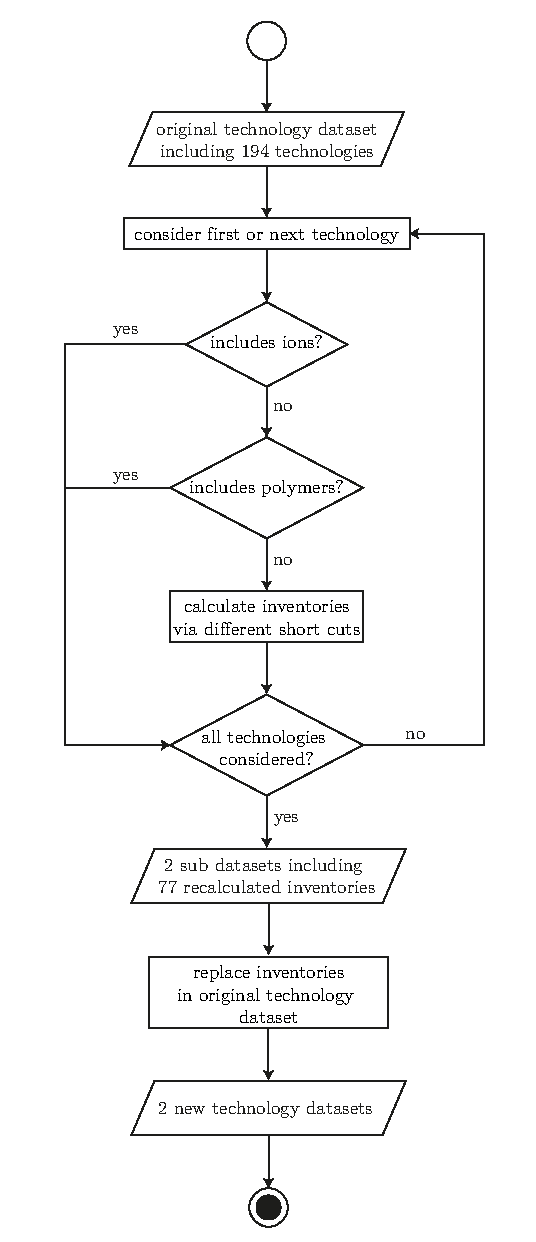
\includegraphics{images/plan_1.pdf}
        \caption{Part one of the model generation process: generating the new sets of inventories}
        \label{fig:plan_1}
\end{figure}

The core of the model underlying the LCA database are the 194 engineering-level technology datasets, each including mass and energy flows, characterizing the chemical processes used for the production of intermediates and the 51 chemicals referred to beforehand. These energy and mass flows are used as inventories of these processes for the calculation of the LCA database. Each one of them is considered individually to determine whether it can be recalculated using the automated \aclp{spdm}. These methods rely on thermodynamic properties such as their temperature-dependant enthalpy $h = h(T)$ and the standard enthalpy of formation $\Delta_f h^\standardstate$ to calculate reaction enthalpies used to estimate heat demands. These values can be determined using COSMO-RS, an equilibrium thermodynamics model and theory used to calculate chemical potentials of molecules in solutions \cite{Klamt.1995}. These are then used to calculate other thermodynamical properties. However, this method leads to high errors when used for ionic solutions, making the set of parameters used for the calculations a subject of recurring scientific publications \cite{Han.2018, Liu.2018}. For polymers, the procedure used by COSMO-RS cannot be applied due to the size of these chemical compounds. Alternatives exist, but report significant errors \cite{SoftwareforChemistry&Materials.2020}. Therefore, processes including ions and polymers are excluded from this study. If the process is not excluded from recalculation, its inventory is then determined with the two methods used in this study. This yields two sub datasets with 77 recalculated inventories. Each dataset including inventories calculated with one of the two \aclp{spdm}. Subsequently, these inventories replace the original ones in the LCA database. The second part starts with these new technology datasets as depicted in Figure \ref{fig:plan_2}.


\begin{figure}[htp]
        \centering
        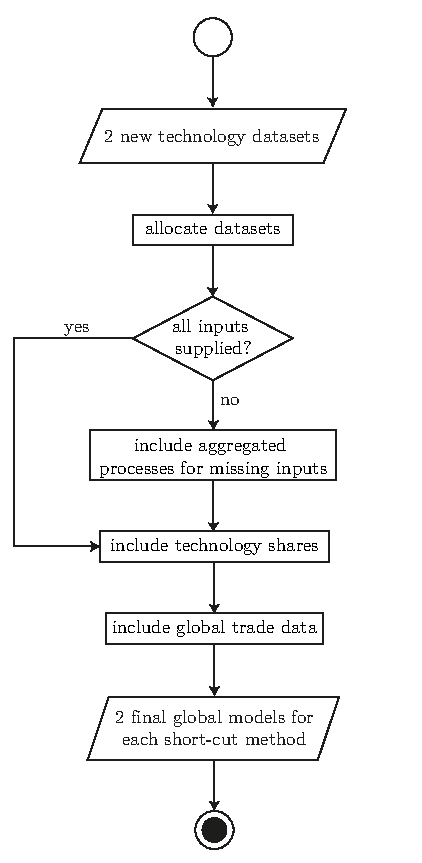
\includegraphics{images/plan_2.pdf}
        \caption{Part two of the model generation process: generating the new models}
        \label{fig:plan_2}
\end{figure}

The technology datasets are then allocated to solve the problem of multifunctionality, so that individual \aclp{GWI} for each chemical product can be calculated. The systems are then checked to identify whether all needed inputs are supplied. If there are unsupplied inputs, supply processes are added successively from the Ecoinvent database \cite{Ecoinvent.2020}. The production processes producing the same chemicals are then set to do so in fixed shares that reflect the real values varying from country to country. As the model also includes a global trade system, these trade flows are then added to the system. Thereby, two complete LCA databases are created, each modeling the worldwide chemical industry, but on the basis of different technology data.
\vspace{2cm}


\section{Applied Simplified Process Design Methods}

The individual methods used in this case study have all been described in detail in Chapter \ref{analysis-spdm}. However, the complete methods used in this case study are a combination of several \aclp{spdm} and are therefore defined in this Chapter.

\paragraph{Method 1: Stoichiometric Mass Flows and Reaction Enthalpy}
In the first method, the stoichiometric equations of the chemical processes are used with a yield of 95 \%, as described in Chapter \ref{stoichiometry}, and suggested by Hischier et. al. \cite{Hischier.2005} and the general rule of thumb proposed by Wells \cite{Wells.1991}. This yields the mass flows. Unconverted reactants are burned, creating direct emissions of the process. The heat use of the process is assumed to equal the reaction enthalpy of the process. The electric energy use is set to be the energy needed for pumps to supply the cooling water needed for the cooling of the reactor according to the reaction enthalpy.


\paragraph{Method 2: Stoichiometric Mass Flows and Ecoinvent's Default Energy Values}
The second method is a reproduction of the estimates used by Ecoinvent \cite{Hischier.2005} in case of few known information about a chemical process, as described in Chapter \ref{gendorf}. Mass inputs are stoichiometric with a yield of 95 \% and subsequent burning of unreacted educts. As default energy values, a use of 2 MJ steam and 0.33 kWh electric energy per kg of output chemical are estimated as suggested by Hischier et. al. \cite{Hischier.2005}. In contrast to the above mentioned method, no fugitive emissions are taken into account.





\chapter{Results and Discussion}
% decide: stoichiometry model/ terminology for the two models and correct in chapter 4
\label{chap:results}
In this chapter, the results of the implementation of \aclp{spdm} will be analysed and discussed. Results will be compared on two different levels: both the recalculated inventories and the \aclp{GWI} of processes and products will be taken into account.


\section{Comparison of Inventories of Production Processes}
\label{sec:inventories}
First, the inventories of the recalculated production processes will be compared. More specifically, the total heat use and the reactant mass flows will be analysed.

\subsection{Total Heat Use}
Heat in chemical processes is assumed to equal the sum of the energetic values of steam and natural gas passing the system boundary of the single chemical process as both represent the most important energy sources for heat generation in chemical processes \cite{Boustead.1999}. Steam is assumed to have a specific energy content of 2.75 MJ/kg \cite{Althaus.2007}. The criterion of heat is used, for it is a major driver of the \acl{GWI} of chemical products. 42 \% of the carbon feedstock used by the chemical industry is used to generate process energy by incineration \cite{InternationalEnergyAgency.2017}, thereby causing the emission of \aclp{GHG}. Simplified process design methods can only be used to calculate the required heat for a process, but not its form, neither its temperature level \cite{Parvatker.2019}. Therefore, this unspecified heat was assumed to be comparable to the combined natural gas and steam use of the industry datasets. Figure \ref{fig:inventories} shows the results of this analysis. Positive values indicate an output of energy, while negative values refer to an energy input. 

\begin{figure}[htp!]
        \centering
        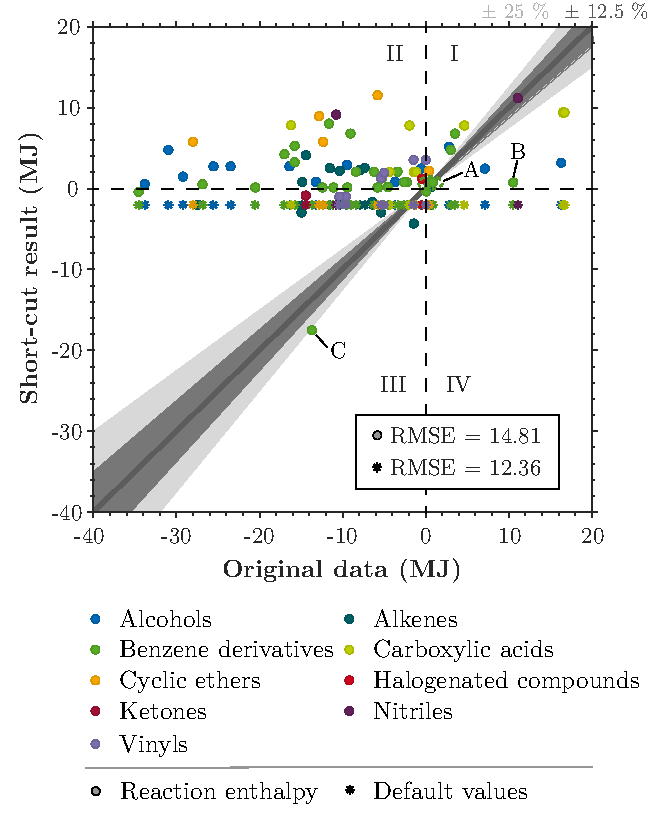
\includegraphics{images/figure_1_clean.pdf}
        \caption{Comparison of the original and recalculated energy output values assumed as steam and natural gas required per one kg of main product. (A) and  (B) mark ethylene- and benzene-based production processes for ethylbenzene with low and high errors, respectively. (C) marks another production process for ethylbenzene that is ethane-based. RMSE refers to the root-mean-square error.}
        \label{fig:inventories}
\end{figure}

\paragraph{Method 1: Stoichiometric Mass Flows and Reaction Enthalpy}
There does not seem to be an overall correlation between the chemical groups and their respective errors. 
\subparagraph{Quadrant I} 
Both the short-cut and original values for the energy outputs are positive. Few points lie in this area in total. Single results are near the 50 \% variance range. One result matches almost perfectly the original value with an error of 0.5 \%: a propane-based acrylonitrile production process. The accumulation of three benzene derivative points near the coordinate origin marked with a dashed green line and the letter A in Figure \ref{fig:inventories} represents three ethylbenzene production processes. All of them have the same underlying stoichiometric formula and therefore form a horizontal line at the value of 0.76 MJ/kg, which means that the underlying reaction is exothermic as the values of method one equal the reaction enthalpy\footnote{it is explicitly remarked that the sign definition of the reaction enthalpy is contrary of the one used in inventories and in Figure \ref{fig:inventories}.}. The original datasets, however, are widely spread: tree of them match this value with relatively low errors (-51.5 \%,	-62.4 \%	 and 13.4 \%, respectively) while another process (B) has an original energy value of 10.54 MJ/kg. While the processes (A) require natural gas and have an output of steam in similar value ranges due to the internal incineration of residuals as fuel, the process (B) both delivers high amounts of natural gas and steam with a value that is more than one order of magnitude higher than the reaction enthalpy of the underlying process. While this process operates at much lower temperature and pressure levels than the processes (A) and therefore, less energy is used internally for heating and pressurizing, it is still a surprisingly high value that, when considering the energy balance of the process, can only be achieved if the inputs have a much higher temperature than the products in the effluent stream. This might be the case in a specific chemical production facility that is interlinked with upstream processes that deliver the input materials at high temperatures as a result of the previous reactions.

\subparagraph{Quadrant II}
In this quadrant, the new inventories have an energy output, meaning that the processes are exothermic, while the original processes require an energy input. Most of the points representing the compared inventories are located in this area with overall large discrepancies between the original and the recalculated values. The reason for this likely is the fact that the reactor -- and therefore the reaction enthalpy -- only represents one element of the whole process. Often, heat is needed for distillation and for preheating the reactants to reaction conditions, even if the reaction is exothermic. In this latter case, surplus energy might be integrated to reduce the heat demand. 

An example of this effect is the production of \acl{BPA}. While the underlying stoichiometry results in a reaction enthalpy of 0.14 MJ/kg (and therefore forming a horizontal line), the original values range from -20.5 MJ/kg to -5.72 MJ/kg, depending on the reaction details such as temperatures, pressures, the number of reaction steps and distillation or purifying process steps; although only one synthesis route for the production of \acl{BPA} is industrially used \cite{Fiege.2000}. This underlines the importance of the reaction conditions that should be taken into account when the required energy for a process is estimated, as previously stated by Jiménez-González et. al.  \cite{JimenezGonzalez.2000}.  

\subparagraph{Quadrant III} 
In this area, both the short-cut and original values reflect an overall energy input. This means that these are endothermic reactions. The overall errors in this area are very high. 
One case (marked with the letter C in Figure \ref{fig:inventories}) matches with a relatively low error of 27.9 \%: another production process for ethylbenzene that is ethane-based. The required energy for this highly endothermic reaction with a reaction enthalpy of $\Delta h_R = -17.51$ MJ/kg to take place is supplied to the process in the forms of (\textit{i}) 15.7 MJ/kg steam, natural gas and electric energy and (\textit{ii}) by an excess of the reactants ethane and benzene that are burned internally as reaction residues, thereby providing around 4.5 MJ/kg (lower heating values according to NIST Chemistry WebBook \cite{NationalInstituteofStandardsandTechnology.2018}).

\subparagraph{Quadrant IV} 
Here, the reactions are endothermic, but the industry datasets report an energy output. There is one single case in this area: a dimethyl terephtalate production process using p-xylene. The difference in energy is supplied to the system in the form of electric energy.


\paragraph{Method 2: Stoichiometric Mass Flows and Ecoinvent's Default Energy Values}

As the default value of $-2$ MJ steam per kg output is assumed, the points form a horizontal line. Two results are within the 25 \% range and no additional results are in the 50 \% range, representing 3.6 \% of the overall results. Figure  \ref{fig:histogram} shows the distribution of the combined heat output values assumed as natural gas and steam of the reference datasets. This distribution equals the density of the points of Method 2 in Figure \ref{fig:inventories}. It clearly depicts that the individual values are widely spread, with a standard deviation of 11.34 MJ and a mean value of $-5.98$ MJ. Consequently, using one default value must lead to high errors.

\begin{figure}[htp!]
        \centering
        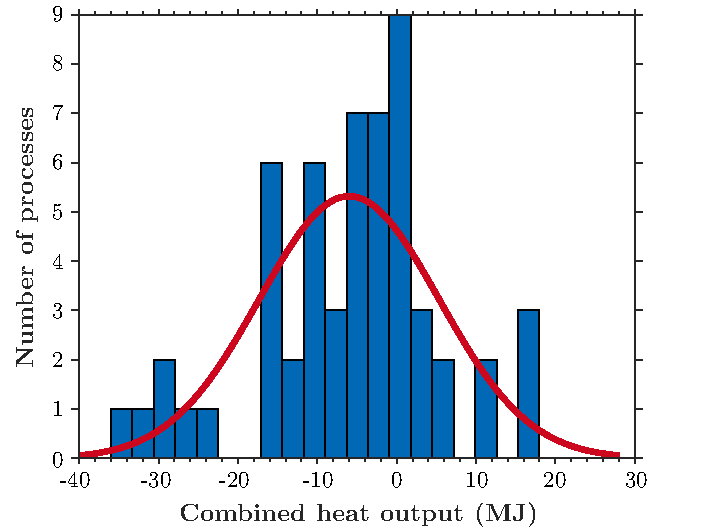
\includegraphics{images/histdist.pdf}
        \caption{Distribution of the combined heat output values assumed as natural gas and steam of the reference datasets}
        \label{fig:histogram}
\end{figure}


\subsection{Reactant Mass Flows}
The following comparison is carried out to assess the accuracy of the estimation of reactant mass flows using stoichiometric equations and the assumption that 5 mass-\% of the inputs are burned. Figure \ref{fig:masses} shows the result of this comparison. Each point refers to an individual mass flow in one process. As both new models use the same method to calculate reactant flows, their results equal.


\begin{figure}[htp!]
        \centering
        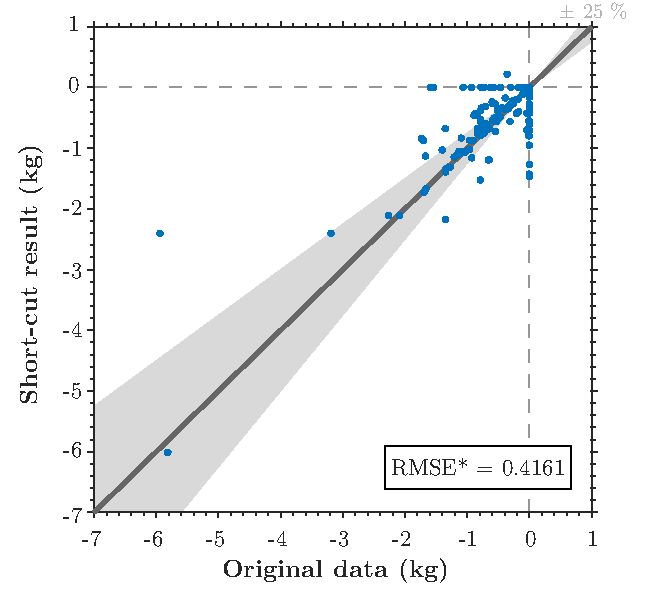
\includegraphics{images/masses.pdf}
        \caption{Comparison of the original and recalculated reactant masses per one kg of main product. The asterisk refers to the set of points not lying on the $x=0$ or $y=0$ lines. RMSE refers to the root-mean-square error.}
        \label{fig:masses}
\end{figure}

40.61 \% of points lie on the $x=0$ or $y=0$ lines. These are cases in which the original model has a mass input, but there is no input of the same chemical in the same process in the new models ($y=0$) and vice-versa. This high percentage of values that only exist in one of the two compared models may indicate several aspects. Firstly and most importantly, the system boundaries of the original and the recalculated processes may not match. This means that the  reactants may differ because of the in- or exclusion of upstream reactions. In the case of very limited data about the reference process, these points may therefore indicate a false synthesis route. Secondly, by-products may be excluded in the reference dataset due to different treatment of these products in industrial processes. 

In one case, the new models have an output of a chemical, while the original dataset uses the same chemical as an input. When only considering non-zero points, the overall derivatives between the estimated mass flows and the original ones are low. 18.38 \% of the points lie within a 5 \% error range, 33.09 \% and 50.74 \% in 10 \% and 25 \% ranges, respectively. For the same set of points, the root-mean-square deviation is 0.4161 kg. 


\section{Comparison of the Impacts of Production Processes}
\label{sec:impacts}

As this thesis is mainly motivated by the need of the chemical industry to reduce its \acl{GHG} emissions, the impact ``ILCD\footnote{The International Reference Life Cycle Data System (ILCD) established by the European Commission, Joint Research Centre, Institute for Environment and Sustainability (JRC - IES) \cite{EuropeanCommissionJointResearchCentreInstituteforEnvironmentandSustainability.2012b}} 1.0.8, 2016, midpoint, climate change, GWP 100a'' \cite{EuropeanCommissionJointResearchCentreInstituteforEnvironmentandSustainability.2012d} was used for the following comparison. The values indicate the \acl{GWI} of an activity\footnote{an activity can be any kind of transformation, production or service defined within the functional unit of the LCA.} in kg CO$_2$-eq based on the characterization factors for elementary flows to the environment published in the Fourth Assessment Report of the Intergovernmental Panel on Climate Change \cite{IPCC.2007}. Inititally, the \aclp{GWI} of all processes included in the database are compared. This comparison is depicted in Figure \ref{fig:impacts all}. Blue dots refer to the model using the reaction enthalpy based model, while red ones refer to the model using Ecoinvent's default energy values.


\begin{figure}[htp!]
        \centering
        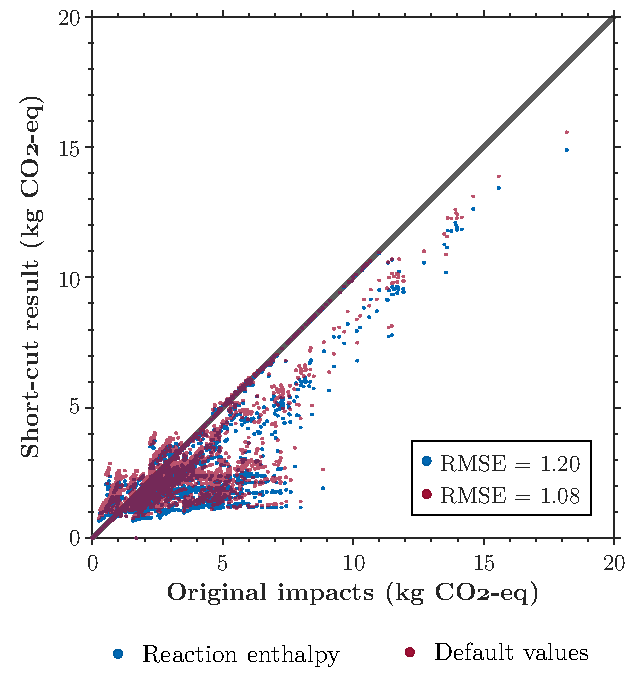
\includegraphics{images/complete_all.pdf}
        \caption{Comparison of all original and recalculated impacts per one kg of main product output included in the ``cm.chemicals'' database \cite{CarbonMindsGmbH.2020}}. RMSE refers to the root-mean-square error.
        \label{fig:impacts all}
\end{figure}

The figure shows that there is a multitude of effects that can be observed with impacts being under- and overestimated in different cases. Some impacts stay equal and seem to be uninfluenced by the changes. The root-mean-square errors of both models are greater than 1 kg CO$_2$-eq with the the second model (RMSE$_2 = 1.08$ kg CO$_2$-eq) performing slightly better than the reaction enthalpy-based model (RMSE$_1 = 1.20$ kg CO$_2$-eq). This means that both models distort the results of the database substantially. To understand some effects in detail, two processes for the production of 1,4-butanediol and vinyl chloride, respectively, will be analysed in detail. For butanediol, a single process based on the reactants acetylene and formaldehyde is studied in detail. It is one of five existing production processes for butanediol.
Figure \ref{fig:butanediol} shows the comparison of the impacts of these five processes. 


\begin{figure}[htp!]
        \centering
        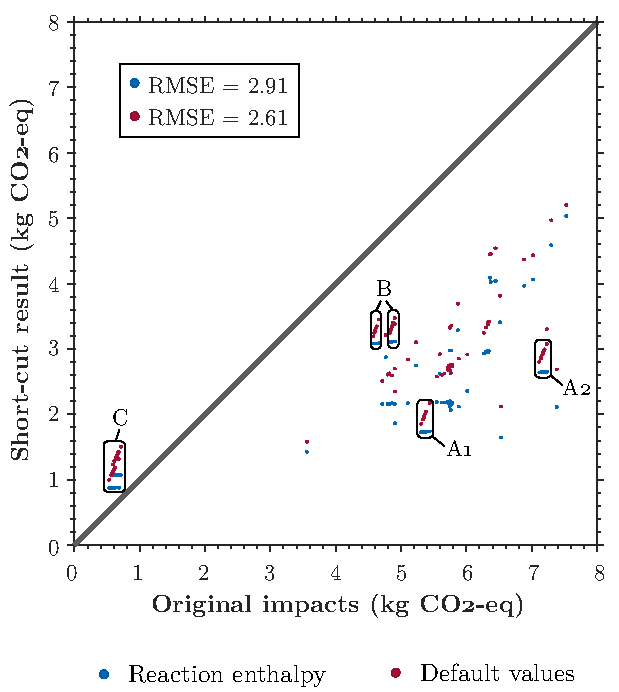
\includegraphics{images/butanediol.pdf}
        \caption{Comparison of the original and recalculated impacts per one kg of 1,4-butanediol for all existing production processes. The letters refer to the following processes: (A) 1,4-butanediol from aetylene and formaldehyde, (B) 1,4-butanediol from maleic anhydride, (C) 1,4-butanediol from butane via maleic acid hydrogenation. RMSE refers to the root-mean-square error.}
        \label{fig:butanediol}
\end{figure}

It can be observed that most impacts are underestimated. There are only a few cases in which the impact is overestimated, all representing the same process. There are patterns or constellations of points representing the different production processes. To understand what the original and recalculated impacts include and why this result is obtained, a contribution analysis in performed. Figure \ref{fig:contribution butanediol} depicts the results of this analysis for two producing regions, Argentina and Belgium, and for the original and two new LCA databases.


\begin{figure}[htp!]
        \centering
        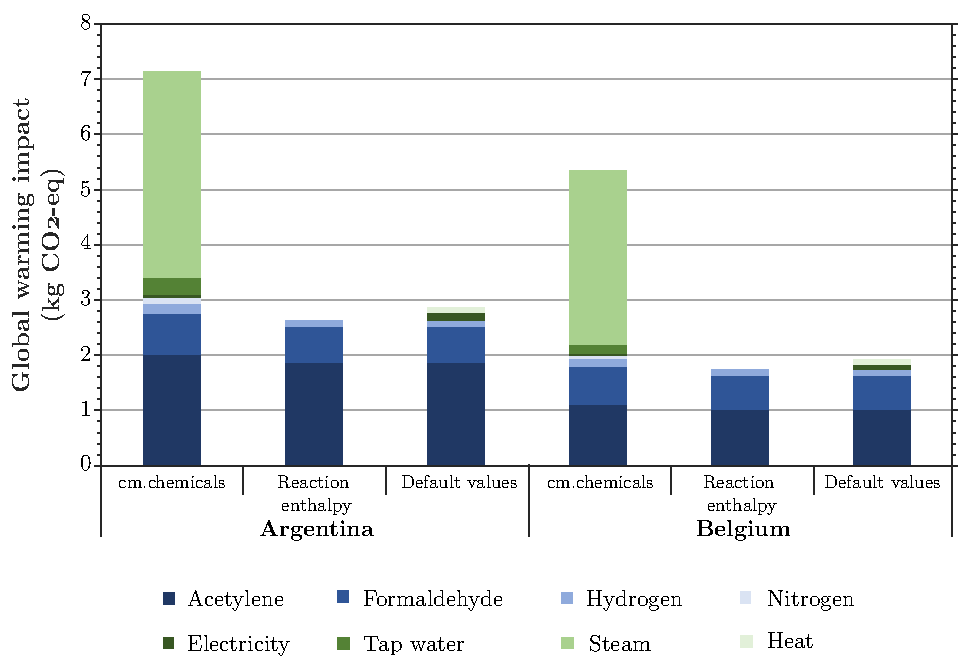
\includegraphics[width=\textwidth]{images/contribution_butanediol.pdf}
        \caption{Contribution analysis of the original and recalculated impacts per one kg of 1,4-butanediol produced by a process based on acetylene and formaldehyde}
        \label{fig:contribution butanediol}
\end{figure}

These results show how the different impacts are composed. Firstly, there is a difference of 1.8 kg CO$_2$-eq between the impacts of the original process when it is used in Argentina compared to its usage in Belgium. This means that in Belgium, the carbon footprint of this production is 25 \% lower. This difference is due to higher impacts of the raw materials acetylene, formaldehyde, hydrogen and nitrogen and the process utilities electricity, tap water, steam and heat. Most importantly, the impact of acetylene is almost twice as high in Argentina than in Belgium. 

In the same country, the impacts calculated using the two new models are by far underestimated when compared to the original impact. The figure also shows that this is mainly due to the drastic underestimation of the steam demand, while reactant-related emissions are very accurate and only almost 10 \% underestimated. 

In the reaction enthalpy based model, the process was calculated to be exothermic. Therefore, the process has undergone allocation, because the surplus energy occurred in the inventory as second output. Additionally, the electricity demand is underestimated. The default heat and electricity values used in the second model are by far too low compared to the real process. Therefore, the impacts are underestimated in both cases.

In all models, all inputs for this process are directly supplied by aggregated  processes from the Ecoinvent database. But these processes only exist for the two regions ``RER'' (Europe) and ``RoW'' (Rest-of-World), except for the electricity supply which exists for most countries individually \cite{Ecoinvent.2020}. This is the reason for similar patterns to occur in Figure \ref{fig:butanediol}. These patterns all represent the same process; but their impact is vastly dependent of their classification regarding the two geographical categories existing in Ecoinvent for the named inputs as has shown the example of Argentina and Belgium. As electricity is the only input that is supplied with processes of high geographical resolution, the points for one model form a line rather than a more complex distribution. It is then its recalculated value that changes the gradient of that line. The closer this value is to the original value, the closer the gradient is to one. This is because, when considering two neighboring points of the same model (A and B) in the same constellation (representing two ``RER'' or ``RoW'' countries, such as two points in the area A$_1$ in Figure \ref{fig:butanediol}), it equals the ratio of the difference in GWI of the new model (on the $y$-axis) divided by the difference in GWI of the original model (on the $x$-axis),
$$
c = \frac{\Delta \mathrm{GWI}_\mathrm{new, \ y}}{\Delta \mathrm{GWI}_\mathrm{original, \ x}}.
$$
These differences equal the difference in GWI of the electricity used because the GWI of all other inputs do equal for both countries in the same region and their deltas are 
$$
\Delta \mathrm{GWI}_i = \sum_j \Delta \mathrm{GWI}_{i, \ j} = \Delta \mathrm{GWI}_{i, \ \mathrm{electricity}},
$$
where $i$ indicates the model used (and can therefore be ``new'' or ``original'') and $j$ refers to the different mass- and energy flows contributing to the total GWI of the process.
The GWI of the electricity used in the same process but in two different countries is the product of the electricity value in the corresponding inventory and the specific GWI of electricity in kg CO$_2$-eq/MJ in the two countries,
$$
\Delta \mathrm{GWI}_{i, \ \mathrm{electricity}} = e_{i} \cdot \left( \mathrm{gwi}_{\mathrm{electricity}, \ \mathrm{A}} - \mathrm{gwi}_{\mathrm{electricity}, \ \mathrm{B}}  \right),
$$
where A and B refer to the neighboring countries. Therefore, the gradient becomes
$$
c = \frac{\Delta \mathrm{GWI}_\mathrm{new, \ y}}{\Delta \mathrm{GWI}_\mathrm{original, \ x}} = \frac{e_{\mathrm{new}} \cdot \left( \mathrm{gwi}_{\mathrm{electricity}, \ \mathrm{A}} - \mathrm{gwi}_{\mathrm{electricity}, \ \mathrm{B}}  \right)}{e_{\mathrm{original}} \cdot \left( \mathrm{gwi}_{\mathrm{electricity}, \ \mathrm{A}} - \mathrm{gwi}_{\mathrm{electricity}, \ \mathrm{B}}  \right)} = \frac{e_{\mathrm{new}}}{e_{\mathrm{original}}}
$$
and therefore can vary in the ranges
$$
c = 
\begin{cases}
c \in [0,1),          & e_\mathrm{original} > e_\mathrm{new} \\
1,                  & e_\mathrm{original} = e_\mathrm{new} \\
c \in (1, \infty),     & e_\mathrm{original} < e_\mathrm{new}.
\end{cases}
$$
This means that if the electricity value is overestimated, the gradient gets larger than one and if it is underestimated, it gets lower than one. 
As the electricity values of the stoichiometry model are near zero, the gradient of the blue lines is also near zero.
The same effect can be found in the data for the production processes of vinyl chloride, as shown in Figure \ref{fig:vinylchloride}.

    
    
\begin{figure}[htp!]
        \centering
        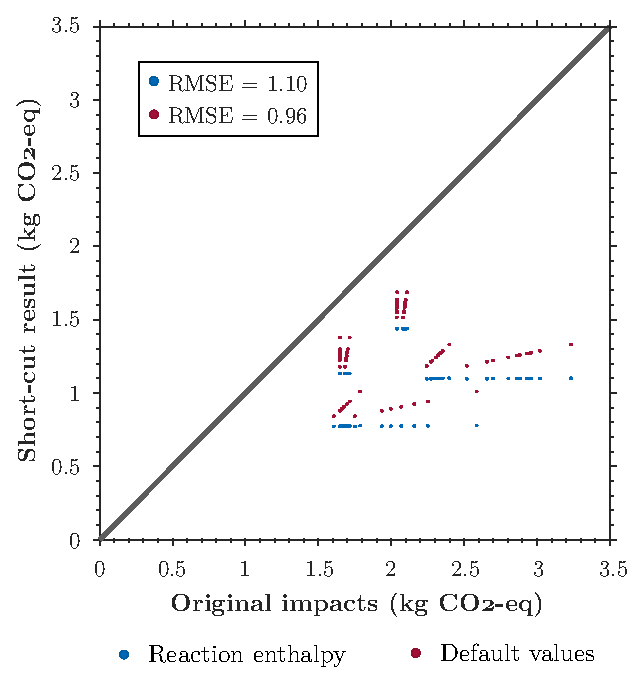
\includegraphics{images/vinylchloride.pdf}
        \caption{Comparison of the original and recalculated impacts per one kg of vinyl chloride for all existing production processes. RMSE refers to the root-mean-square error.}
        \label{fig:vinylchloride}
\end{figure}


As the gradient for one process in one of the two new models can only have one value, the ratio between the recalculated and the original electricity values $c = {e_{\mathrm{new}}}/{e_{\mathrm{original}}}$, it is easily deducible that there must be four production processes for vinyl chloride, as four different gradients appear in Figure \ref{fig:vinylchloride}. Considering the gradients of the red ``lines'', the electric energy value of the underlying simulation model is an underestimate in the case of one process, a good estimate in another process and an overestimate in two processes. 

In the example of vinyl chloride, there is another effect that can be observed. The stoichiometric formulas of the underlying processes all list one or two by-products of the reaction, while the original process has a single output. For example, in a process using ethane, chlorine and hydrogen as reactants, the corresponding stoichiometric formula is \ce{2 C2H6 + 2 Cl2 + O2 -> 2 C2H3Cl + 2 H2O + 2 HCl}, which results in the by-products water and hydrogen chloride. However, in the original dataset, (\textit{i}) none of these by-products are indicated and (\textit{ii}) ethane and oxygen are used in large excess. Both effects result in a non-closed mass balance. Then, in the allocation step, the mass and energy input values are multiplied by the allocation factor ($<1$, because there are by-products) and are therefore much lower for ethane and oxygen than in the original process. This results in fewer emissions related to the production of these two reactants than in the reference dataset, as depicted in Figure \ref{fig:contribution vinylchloride}. The impact of chlorine is almost equal due to the fact that the original dataset's chlorine consumption matches the allocated value of the new datasets. It is likely that ethane is used in excess, because it is burned to provide process heat.

\begin{figure}[htp!]
        \centering
        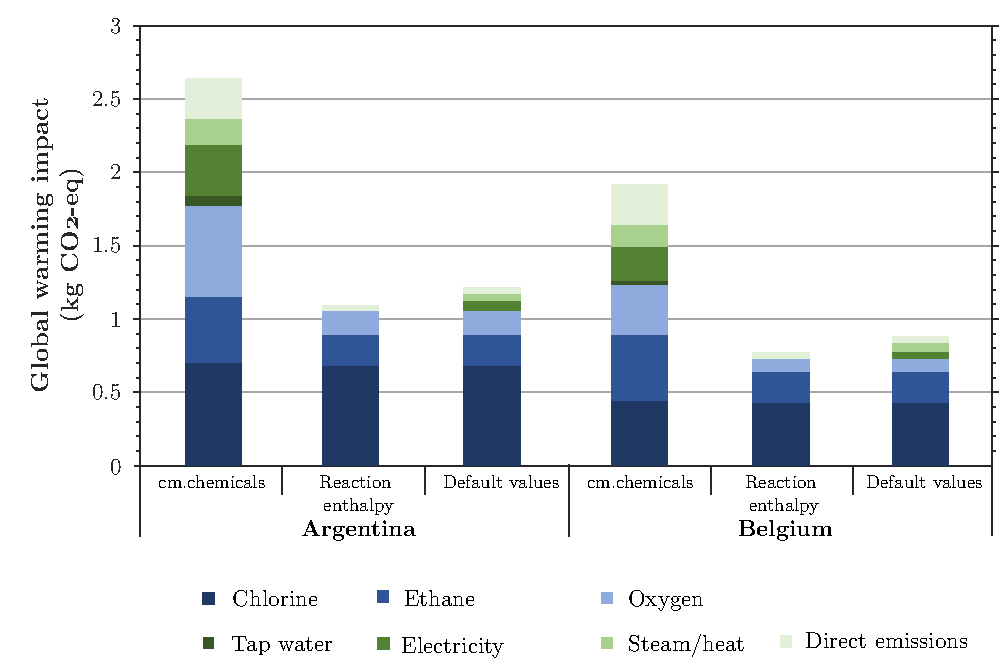
\includegraphics[width=\textwidth]{images/contribution_vinylchloride.pdf}
        \caption{Contribution analysis of the original and recalculated impacts per one kg of vinyl chloride produced by a process based on ethane, oxygen and chlorine}
        \label{fig:contribution vinylchloride}
\end{figure}



\chapter{Conclusions and Outlook}
In this thesis, existing \aclp{spdm} to calculate mass and energy balances for chemical processes have been reviewed. It has been discussed what effects can occur when using these methods in the context of an LCA database framework. Subsequently, a case study has been carried out, applying two methods for the generation of inventories to an existing LCA database of the worldwide chemical industry. The results have been analysed and interpreted with regards to deviation in mass and energy balances as well as global warming impacts for two chemical products.

% Conclusion on LCA and LCA databases (c 2-3) theory
For the inventories generated, the following conclusions can be derived. These include limitations and pitfalls that need to be considered when applying \aclp{spdm} to generate mass and energy balances for chemical production processes to calculate LCA databases.  
\begin{itemize}
    \item A lot of \aclp{spdm} as well as methodologies for the development of inventories have been published and applied in scientific literature to calculate mass and energy flows of chemical processes. In single cases, these have been validated and some implications when carrying out a LCA based on such inventories have been studied. In this thesis, these existing methods have structurally been evaluated qualitatively regarding their implications for mass and energy flows.
    \item The plain stoichiometric method underestimate mass flows and resulting impacts. Taking into account conversion or yield percentages can result in better estimation of the original mass flows.
    \item Calculating heating energy requirements according to the temperature change that has to be achieved provides an accurate tool for the estimation of this part of the heat demand. 
    \item Often, efficiencies $\eta$ used in the calculations decide whether a method over- or underestimates specific flows. It should be ensured that these efficiencies reflect real values as accurately as possible. 
    \item Fugitive emissions are best estimated using the elaborate method of Smith et. al., while the emission factors used by Ecoinvent and Jiménez-González et al. are expected to overestimate fugitive emissions significantly. Besides that, the fugitive emission method by Ecoinvent only accounts for educt emissions, even though intermediates and products
     %If there are assumptions on fugitive and venting emissions, these mostly focus on inputs, but not on intermediates or products, although these 
    might have a higher ecological relevance.%Methodologies existing for the calculation of fugitive emissions should be applied for these chemicals, too.
    \item Often, \aclp{spdm} do not include assumptions for waste flows and subsequent waste treatment. Therefore, emissions released during these stages are not taken into account, leading to an underestimation of the ecologic burdens of a process. The assumption of incineration of all residues is the worst case scenario when analysing greenhouse gas emissions of a process. Analogous assumptions should be used when considering other impact categories.  
    \item Simplified process design methods ignore ancillary materials, such as solvents and catalysts, and their potential ecological burden and therefore underestimate ecologic impacts. When analysing chemical processes, data that reflects these additional mass flows should be collected. 
    \item There are no assumptions for energy demands of additional processing operations such as purifying or crystallisation steps. Thus, for the generation of new LCA databases, developing methods or heuristics for additional process operations might help in the estimation of heat and electricity requirements.
    \item Introducing cut-off has a minor influence if the cut-off is performed properly. It has to be ensured that cut-off does not exclude environmentally relevant flows from the inventory, even though they are below the cut-off limit.
    \item In a more general context, to be able to use \aclp{spdm}, assumptions have to be made that most accurately reflect the real process. For instance, heat sources and synthesis routes have to be determined. When few data about a process is available, taking appropriate assumptions can be difficult.
\end{itemize}



% Conclusion on the results (c5) case study
Based on the results of the case study and in the context of the calculation of ecologic impacts, the following aspects have to be considered:

\begin{itemize}

    \item Most of the impacts of the processes and products included in the database change when using \aclp{spdm} as the production system under study is highly interconnected. For the two methods used in the case study, the root-mean-square error of all global warming impacts included in the database are 1.20 kg CO$_2$-eq and 1.08 kg CO$_2$-eq for the reaction enthalpy based and the default values models, respectively. It has to be pointed out that this occurs, although only about 40 \% of the technology datasets have been recalculated. 
    \item The contribution analysis shows that the energy demands and material inputs are the major driver of the \acl{GWI} of chemical products. Under- or overestimation of these values change their impact accordingly and result in high errors. Especially for the heat used in chemical processes, care has to be taken, because even for the same synthesis routes, heat demands of different processes can vary significantly. In the example of bisphenol A production processes, the industrial heat demands cover the range between $-20.5$~MJ/kg and $-5.72$ MJ/kg. The overall original heat demands of all processes have a standard deviation of 11.34 MJ/kg. This underlines the need for the development of methods taking into account process-specific characteristics and hot spots of heat usage to enable LCA practitioners to estimate appropriate energy demands for chemical processes. Overall, the default value of $-2$~MJ/kg heat performs better than using reaction enthalpies as heat demands, as almost all processes considered need heat, even if they are are exothermic.
    \item Although the used energy requirement calculations perform poor, stoichiometric mass flows matched the original values well with a root-mean-square error of 0.42 kg and more than 50 \% of the points lying within an error range of 25 \%. Nevertheless, it has to be assured that the system boundaries of the original processes are used to recalculate mass flows to represent processes accurately. This might be challenging if few data about processes is available. 
    \item  During allocation, the allocation factors might change depending on whether mass, energy or price is used for their calculation. In the example of the case study, allocation was performed using mass ratios of the products. These might differ to those in industrial data due to differing system boundaries or flows excluded in industrial datasets. Different allocation factors can significantly change the resulting allocated inventories and therefore distort the ecologic impacts of products. Thus, implementing allocation introduces uncertainties into an LCA database.
    \item The regionalisation of the background system used to supply the model's inputs influences the results decisively. In the case study, several impacts doubled for regions classified as ``Rest-of-World'', while the real impact may be lower in the specific countries.
    \item The case study shows that there is a large variety of effects that occur when using \aclp{spdm} to generate \ac{LCA} databases. Some of them have been studied in this thesis, but more are to be understood in detail so that robust LCA studies for chemical products may be carried out.
\end{itemize}

The methods used in the case study are appropriate to calculate mass flows for chemical LCA databases. However, due to the large errors, they should not be used to calculate energy flows. Thus, to evaluate chemical products environmentally, the used \aclp{spdm} do not provide sufficient accuracy for the generation of a LCA database. In further research, the used set of \aclp{spdm} can be altered and validated to enable correct, fast and automated LCA database generation and to facilitate chemical LCAs. This could contribute to delivering reliable information for decision makers on how to decrease the greenhouse gas emissions of the chemical industry to mitigate anthropogenic climate change. 



\appendix

\chapter{Appendix: Fugitive Emission Methods}
\section{Comparison of the Fugitive Emission Methods by Smith et al. \cite{Smith.2017}, Jiménez-González et al. \cite{JimenezGonzalez.2000} and Ecoinvent \cite{Hischier.2005}}

Assuming the method of Smith et al. to be afflicted with small error (see Chapter \ref{chap:Smith}), the methods by Jiménez-González et al. and Ecoinvent can be evaluated by a  comparison to the method by Smith et al.

Table \ref{tab:comp-fugi} and \ref{tab:comp-fugi-Eco} document the calculations to make the three approaches comparable. Based on the generic flow sheet (Figure \ref{fig:flow sheet}), a number of three compressors or pumps is assumed. As the emission factors by Smith et al. are time dependent, a substance flow of 1000 $\frac{\mathrm{kg}}{\mathrm{h}}$ is assumed, based on the assumption of 1000 $\frac{\mathrm{kg}}{\mathrm{h}}$ product flow in the case study in \cite{JimenezGonzalez.2000}. To make the emission factors comparable, the emission factors by Smith et al. need to be multiplied by the number of pumps or compressors and divided by the substance mass flow. This results in comparable emission factors.

The result of the first comparison (Table \ref{tab:comp-fugi}) is that the emission factors by Jiménez-González at al. for light liquids, heavy liquids and gases are two magnitudes, three magnitudes and one magnitude higher than the factors in the method by Smith et al.

The result of the second comparison (Table \ref{tab:comp-fugi-Eco}) is that the emission factor by Ecoinvent  is two magnitudes, three magnitudes and one magnitude higher than the factors in the method by Smith et al. for light liquids, heavy liquids and gases.

\begin{table}[]
    \caption[Comparison of the fugitive emission factors 1]{Comparison of the fugitive emission methods by Smith et al. \cite{Smith.2017} and Jiménez-González et al. \cite{JimenezGonzalez.2000}. Jiménez-González et al. distinguish fluids according to the boiling point at 1013 hPa: light liquids: $20...60$ °C; heavy liquids $60...120$ °C. Smith et al. distinguish fluids according to the vapor pressure at 20 °C: light liquids $>0.3$ kPa; heavy liquids $<0.3$ kPa.}
    \label{tab:comp-fugi}
    \centering
    \resizebox{\textwidth}{!}{
    \begin{tabular}{cccc}\toprule
\textbf{fluid}   &\multicolumn{2}{c}{\textbf{emission factors by}}            &\textbf{difference} \\
 {}     &\textbf{Smith et al.}           & \textbf{Jiménez-González et al.}   & {}        \\\midrule
light liquid    &   $3\cdot 0.0199 \frac{\mathrm{kg}}{\mathrm{h}\cdot \mathrm{source}}=0.0597 \frac{\mathrm{kg}}{\mathrm{h}}$ &               &  \\
                &   $\frac{0.0597 \ \mathrm{kg/h}}{1000 \ \mathrm{kg/h}}=0.00597 \%$                   &   $2 \ \%$       &3 magnitudes\\\midrule
heavy liquid    &   $3\cdot 0.00862 \  \frac{\mathrm{kg}}{\mathrm{h}\cdot \mathrm{source}}=0.02586 \frac{\mathrm{kg}}{\mathrm{h}}$&               & \\
                &   $\frac{0.02586 \ \mathrm{kg/h}}{1000 \ \mathrm{kg/h}}=0.002586 \%$                &   $1 \ \%$ & 3 magnitudes\\\midrule
gases           &  $3\cdot 0.288 \  \frac{\mathrm{kg}}{\mathrm{h}\cdot \mathrm{source}}=0.864  \frac{\mathrm{kg}}{\mathrm{h}}$ & & \\
           & $\frac{0.864 \ \mathrm{kg/h}}{1000 \ \mathrm{{kg/h}}}=0.0864 \%$ & $0.5 \ \%$ & 1 magnitude\\\bottomrule
\end{tabular}}
\end{table}

\begin{table}[]
    \caption[Comparison of the fugitive emission factors 2]{Comparison of the fugitive emission methods by Smith et al. \cite{Smith.2017} and Ecoinvent \cite{Hischier.2005}. Smith et al. distinguish fluids according to the vapor pressure at 20 °C: light liquids $>0.3$ kPa; heavy liquids $<0.3$ kPa.}
    \label{tab:comp-fugi-Eco}
    \centering
    \resizebox{\textwidth}{!}{
    \begin{tabular}{cccc}\toprule
\textbf{fluid} &\multicolumn{2}{c}{\textbf{emission factors by}} & \textbf{}\\
   &    \textbf{Smith et al.}    & \textbf{Ecoinvent emission } & \textbf{difference}\\\midrule
light liquid    &   $3\cdot 0.0199 \frac{\mathrm{kg}}{\mathrm{h}\cdot \mathrm{source}}=0.0597 \frac{\mathrm{kg}}{\mathrm{h}}$ &               &  \\
                &   $\frac{0.0597 \ \mathrm{kg/h}}{1000 \ \mathrm{kg/h}}=0.00597 \%$                 &   $0.2 \ \%$       &2 magnitudes\\\midrule
heavy liquid    &   $3\cdot 0.00862 \  \frac{\mathrm{kg}}{\mathrm{h}\cdot \mathrm{source}}=0.02586 \frac{\mathrm{kg}}{\mathrm{h}}$&               & \\
                &   $\frac{0.02586 \ \mathrm{kg/h}}{1000 \ \mathrm{kg/h}}=0.002586 \%$                 &   $0.2 \ \%$ & 2 magnitudes\\\midrule
gases           &  $3\cdot 0.288 \  \frac{\mathrm{kg}}{\mathrm{h}\cdot \mathrm{source}}=0.864  \frac{\mathrm{kg}}{\mathrm{h}}$ & & \\
           & $\frac{0.864 \ \mathrm{kg/h}}{1000 \ \mathrm{{kg/h}}}=0.0864 \%$ & $0.2 \ \%$ & 1 magnitude\\\bottomrule
\end{tabular}}
\end{table}

\chapter{Appendix: Details on the cm.chemicals Database}
\label{appA}


\section{Chemical Products Included in the ``cm.chemicals'' Database}



\begin{longtable}[c]{@{}ll@{}}
\caption{Chemical products included in the ``cm.chemicals'' database provided by Carbon Minds GmbH as of the 27th of April 2020 \cite{CarbonMindsGmbH.2020}}
\label{tab:chemicals}\\
\toprule
\textbf{Chemical}                         & \textbf{CAS-Number} \\* \midrule
\endfirsthead
%
\multicolumn{2}{c}%
{{\bfseries Table \thetable\ continued from previous page}} \\
\toprule
\textbf{Chemical}                         & \textbf{CAS-Number}  \\* \midrule
\endhead
%
\bottomrule
\endfoot
%
\endlastfoot
%
1,4-Butanediol                   & 000110-63-4 \\
ABS resin                        & 009003-56-9 \\
Acetic acid                      & 000064-19-7 \\
Acetone                          & 000067-64-1 \\
Acrylic acid                     & 000079-10-7 \\
Acrylonitrile                    & 000107-13-1 \\
Aniline                          & 000062-53-3 \\
Benzene                          & 000071-43-2 \\
Bisphenol A                      & 000080-05-7 \\
Butadiene                        & 000106-99-0 \\
Butyl rubber                     & 009010-85-9 \\
Cumene                           & 000098-82-8 \\
Demethyl therephthalate          & 000120-61-6 \\
Dinitrotoluene                   & 000121-14-2 \\
Diphenyl carbonate               & 000102-09-0 \\
EPDM rubber                      & 308064-28-0 \\
Ethylbenzene                     & 000100-41-4 \\
Ethylene                         & 000074-85-1 \\
Ethylene glycol                  & 000107-21-1 \\
Ethylene oxide                   & 000075-21-8 \\
Hexene-1                         & 000592-41-6 \\
Isobutanol                       & 000078-83-1 \\
Isopropanol                      & 000067-63-0 \\
Methanol                         & 000067-56-1 \\
Methylene diphenyl isocyanate    & 000101-68-8 \\
N-Butanol                        & 000071-36-3 \\
N-Butyraldehyde                  & 000123-72-8 \\
Octene-1                         & 000111-66-0 \\
Olefins, linear alpha            & unspecific  \\
O-Xylene                         & 000095-47-6 \\
PET pellets (IV=0.6)             & 025038-59-9 \\
Phenol                           & 000108-95-2 \\
Polycarbonate                    & unspecific  \\
Polyether Polyol (trifunctional) & unspecific  \\
Polyethylene, HD                 & 009002-88-4 \\
Polyethylene, LD                 & 009002-88-4 \\
Polyethylene, LLD                & 009002-88-4 \\
Polypropylene                    & 009003-07-0 \\
Polystyrene, expandable          & 009003-53-6 \\
Polystyrene, general purpose     & 009003-53-6 \\
Polyvinyl chloride               & 000075-01-4 \\
Propylene                        & 000115-07-1 \\
Propylene oxide                  & 000075-56-9 \\
P-Xylene                         & 000106-42-3 \\
Styrene                          & 000100-42-5 \\
Terephthalic acid                & 000100-21-0 \\
Toluene                          & 000108-88-3 \\
Toluene diisocyanate             & 000091-08-7 \\
Vinyl acetate                    & 000108-05-4 \\
Vinyl chloride                   & 000075-01-4 \\
Xylenes, mixed                   & unspecific  \\* \bottomrule
\end{longtable}



\section{Countries Included in the ``cm.chemicals'' Database}


\begin{longtable}[c]{@{}ll@{}}
\caption{Countries included in the ``cm.chemicals'' database provided by Carbon Minds GmbH as of the 27th of April 2020 \cite{CarbonMindsGmbH.2020}}
\label{tab:countries}\\
\toprule
\textbf{Name}  & \textbf{ISO-3166 Code} \\* \midrule
\endfirsthead
%
\multicolumn{2}{c}%
{{\bfseries Table \thetable\ continued from previous page}} \\
\toprule
\textbf{Name}  & \textbf{ISO-3166 Code} \\* \midrule
\endhead
%
\bottomrule
\endfoot
%
\endlastfoot
%
Argentina      & AR                     \\
Belgium        & BE                     \\
Brazil         & BR                     \\
Canada         & CA                     \\
China          & CN                     \\
France         & FR                     \\
Germany        & DE                     \\
India          & IN                     \\
Iran           & IR                     \\
Italy          & IT                     \\
Japan          & JP                     \\
Malysia        & MY                     \\
Mexico         & MX                     \\
Poland         & PL                     \\
Russia         & RU                     \\
Saudi Arabia   & SA                     \\
Singapore      & SG                     \\
South Korea    & KR                     \\
Spain          & ES                     \\
Taiwan         & TW                     \\
Thailand       & TH                     \\
United Kingdom & GB                     \\
United States  & US                     \\* \bottomrule
\end{longtable}


\section{Ecoinvent Processes Used to Supply Production Processes}
\label{app:ecoinvent}
% Please add the following required packages to your document preamble:
% \usepackage{booktabs}
% \usepackage{longtable}
% Note: It may be necessary to compile the document several times to get a multi-page table to line up properly
\begin{longtable}[c]{@{}ll@{}}
\caption{Allocated Ecoinvent activities \cite{Ecoinvent.2020} used as supplies for production processes}
\label{tab:ecoinvent}\\
\toprule
\textbf{Ecoinvent Activity Name}       & \textbf{Flow Supplied}      \\* \midrule
\endfirsthead
%
\multicolumn{2}{c}%
{{\bfseries Table \thetable\ continued from previous page}} \\
\toprule
\textbf{Ecoinvent Activity Name}       & \textbf{Flow Supplied}      \\* \midrule
\endhead
%
\bottomrule
\endfoot
%
\endlastfoot
%
\begin{tabular}[c]{@{}l@{}}market for ammonia,\\   liquid\end{tabular} &
  ammonia, liquid \\
market for butane                      & butane                      \\
market for butene, mixed               & butene, mixed               \\
\begin{tabular}[c]{@{}l@{}}market for calcium carbide, technical\\   grade\end{tabular} &
  calcium carbide, technical grade \\
market for carbon dioxide, liquid      & carbon dioxide, liquid      \\
market for carbon monoxide             & carbon monoxide             \\
market for chemicals, inorganic        & chemical, inorganic         \\
chemical production, organic           & chemical, organic           \\
market for chemical, organic           & chemical, organic           \\
market for chlorine, liquid            & chlorine, liquid            \\
market for electricity, medium voltage & electricity, medium voltage \\
market for ethane                      & ethane                      \\
\begin{tabular}[c]{@{}l@{}}market for ethanol, without water, in \\ 99.7\% solution state, from fermentation\end{tabular} &
  \begin{tabular}[c]{@{}l@{}}ethanol, without water, in \\ 99.7\% solution state, from fermentation\end{tabular} \\
market for ethylene dichloride         & ethylene dichloride         \\
market for formaldehyde                & formaldehyde                \\
\begin{tabular}[c]{@{}l@{}}market group for heat, district or\\   industrial, natural gas\end{tabular} &
  heat, district or industrial, natural gas \\
market for heavy fuel oil              & heavy fuel oil              \\
market for hexane                      & hexane                      \\
\begin{tabular}[c]{@{}l@{}}market for hydrochloric acid, without\\ water, in 30\% solution state\end{tabular} &
  \begin{tabular}[c]{@{}l@{}}hydrochloric acid, without \\ water, in 30\% solution state\end{tabular} \\
market for hydroquinone                & hydroquinone                \\
market for isobutanol                  & isobutanol                  \\
market for lignite                     & lignite                     \\
market for maleic anhydride            & maleic anhydride            \\
market for methylchloride              & methylchloride              \\
market for natural gas, high pressure  & natural gas, high pressure  \\
\begin{tabular}[c]{@{}l@{}}market for nitric acid, without water, in\\ 50\% solution state\end{tabular} &
  \begin{tabular}[c]{@{}l@{}}nitric acid, without water, in \\ 50\% solution state\end{tabular} \\
market for nitrobenzene                & nitrobenzene                \\
market for nitrogen, liquid            & nitrogen, liquid            \\
pentane production                     & pentane                     \\
market for petroleum coke              & petroleum coke              \\
market for polybutadiene               & polybutadiene               \\
market for propane                     & propane                     \\
market for quicklime, milled, loose    & quicklime, milled, loose    \\
\begin{tabular}[c]{@{}l@{}}market for sodium hydroxide, without\\ water, in 50\% solution state\end{tabular} &
  \begin{tabular}[c]{@{}l@{}}sodium hydroxide, without \\ water, in 50\% solution state\end{tabular} \\
market for sulfuric acid               & sulfuric acid               \\
market for synthetic gas               & synthetic gas               \\
market for tap water                   & tap water                   \\
market for trichloromethane            & trichloromethane            \\
\begin{tabular}[c]{@{}l@{}}market for water, deionised, from tap\\   water, at user\end{tabular} &
  water, deionised, from tap water, at user \\* \bottomrule
\end{longtable}














% bibliography
\setlength{\emergencystretch}{3em}
\printbibliography


\end{document}